\documentclass{article}

% if you need to pass options to natbib, use, e.g.:
% \PassOptionsToPackage{numbers, compress}{natbib}
% before loading nips_2016
%
% to avoid loading the natbib package, add option nonatbib:
% \usepackage[nonatbib]{nips_2016}

\usepackage[final]{nips_2016_modified}

% to compile a camera-ready version, add the [final] option, e.g.:
% \usepackage[final]{nips_2016}

\usepackage[utf8]{inputenc} % allow utf-8 input
\usepackage[T1]{fontenc}    % use 8-bit T1 fonts
\usepackage{hyperref}       % hyperlinks
\usepackage{url}            % simple URL typesetting
\usepackage{nicefrac}       % compact symbols for 1/2, etc.
\usepackage{microtype}      % microtypography
%% dritchie: I already have these in my packages.tex
% \usepackage{booktabs}       % professional-quality tables
% \usepackage{amsfonts}       % blackboard math symbols

% -- dritchie preamble modifications ------------------------------------------

%% Packages I've found useful over the years
%auto-ignore
% \usepackage[usenames,dvipsnames]{xcolor}
\usepackage{amsmath,listings,xspace,color,amssymb}
\usepackage{amsfonts}
\usepackage{dsfont}
\usepackage{enumitem}
\usepackage{mathtools}
\usepackage{bm}

%% Better font for code blocks
\usepackage{inconsolata}

%% For auto-inserting line breaks in extra long equations
\usepackage{etoolbox}
\usepackage{breqn}

% Specifying reft/left alignment of figures
\usepackage[export]{adjustbox}

%% For algorithm pseudocode listings
\usepackage{algorithm}
\usepackage[noend]{algpseudocode}

%% Advance theorem/proof formatting
\usepackage{amsthm}

% Yo dawg, I heard you like figures...
\usepackage{subcaption}
% arXiv has problems if I don't do this
\captionsetup{compatibility=false}

%% Because dmath and line numbering don't play well together
% See http://tex.stackexchange.com/questions/86529/breqn-and-lineno-incompatibility
\BeforeBeginEnvironment{dmath}{\begin{nolinenumbers}}
\AfterEndEnvironment{dmath}{\end{nolinenumbers}}
\BeforeBeginEnvironment{dmath*}{\begin{nolinenumbers}}
\AfterEndEnvironment{dmath*}{\end{nolinenumbers}}

\usepackage{booktabs}
\usepackage{multirow}
\usepackage{array}

\usepackage[percent]{overpic}

\usepackage{wrapfig}

\usepackage{bm}

%% Macros and other useful commands/shorthand
%auto-ignore
%% For adding comments to the text
\newcommand{\remark}[1]{\textcolor{red}{[#1]}}
% \newcommand{\remark}[1]{}

%% Vector quantities
\newcommand{\vecstyle}[1]{\mathbf{#1}}

\newcommand{\specialcell}[2][c]{%
  \begin{tabular}[#1]{@{}l@{}}#2\end{tabular}}

%% Units of measurement
\newcommand{\unit}[1]{\ensuremath{\,\mathrm{#1}}}

%% The indicator function
\newcommand{\indicator}[1]{\ensuremath{\mathds{1}\{#1\}}}

%% The normal distribution
\newcommand{\normdist}{\ensuremath{\mathcal{N}}}

%% KL divergence
\newcommand{\KLD}{\ensuremath{D_{\text{KL}}}}

%% The set of real numbers
\newcommand{\Rn}{\ensuremath{\mathds{R}^n}}

%% Inline code listings
\newcommand{\ic}[1]{\lstinline[basicstyle=\fontsize{8pt}{8.25pt}\selectfont\ttfamily]{#1}}

%% Notation that's specific to this paper
%auto-ignore

\newcommand{\latentVar}{\ensuremath{x}}
\newcommand{\observedVar}{\ensuremath{y}}
\newcommand{\latentVars}{\ensuremath{\vecstyle{\latentVar}}}
\newcommand{\observedVars}{\ensuremath{\vecstyle{\observedVar}}}

% -------------------------------------------------------------------

\newcommand{\trueJoint}{\ensuremath{p(\latentVars, \observedVars)}}
\newcommand{\trueJointPhi}{\ensuremath{p(\latentVars, \observedVars ; \phi)}}
\newcommand{\trueJointTheta}{\ensuremath{p(\latentVars, \observedVars; \theta)}}

\newcommand{\truePosterior}{\ensuremath{p(\latentVars | \observedVars)}}
\newcommand{\truePosteriorPhi}{\ensuremath{p(\latentVars | \observedVars ; \phi)}}
\newcommand{\truePosteriorTheta}{\ensuremath{p(\latentVars | \observedVars ; \theta)}}

\newcommand{\dataMarginal}{\ensuremath{p(\observedVars)}}
\newcommand{\dataMarginalPhi}{\ensuremath{p(\observedVars ; \phi)}}
\newcommand{\dataMarginalTheta}{\ensuremath{p(\observedVars ; \theta)}}

% -------------------------------------------------------------------

% \newcommand{\guide}{\ensuremath{g}}
\newcommand{\guide}{\ensuremath{q}}

\newcommand{\guidePosterior}{\ensuremath{\guide(\latentVars | \observedVars ; \phi)}}
\newcommand{\guidePostNoPhi}{\ensuremath{\guide(\latentVars | \observedVars)}}

\newcommand{\elbo}{\ensuremath{\mathcal{L}(\observedVars)}}
\newcommand{\elboPhi}{\ensuremath{\mathcal{L}(\observedVars, \phi)}}
\newcommand{\elboPhiTheta}{\ensuremath{\mathcal{L}(\observedVars, \phi, \theta)}}

\newcommand{\elboDef}{\ensuremath{\expect_{\guide}[ \log \trueJoint - \log \guidePosterior ]}}
\newcommand{\elboDefGenPhi}{\ensuremath{\expect_{\guide}[ \log \trueJointPhi - \log \guidePosterior ]}}
\newcommand{\elboDefGenTheta}{\ensuremath{\expect_{\guide}[ \log \trueJointTheta - \log \guidePosterior ]}}

\newcommand{\gradparams}{\ensuremath{\nabla_\phi}}
\newcommand{\gradparamsTheta}{\ensuremath{\nabla_\phi}}

% -------------------------------------------------------------------

\newcommand{\reparamVar}{\ensuremath{\epsilon}}
\newcommand{\reparamVars}{\ensuremath{\bm{\epsilon}}}
\newcommand{\reparamDist}{\ensuremath{r}}
\newcommand{\reparamXform}{\ensuremath{g}}
\newcommand{\xformedVar}{\ensuremath{\reparamXform(\reparamVar)}}
\newcommand{\xformedVarPhi}{\ensuremath{\reparamXform(\reparamVar ; \phi)}}
\newcommand{\xformedVars}{\ensuremath{\reparamXform(\reparamVars)}}
\newcommand{\xformedVarsPhi}{\ensuremath{\reparamXform(\reparamVars ; \phi)}}




%% Code examples in this paper will be in Javascript or WebPPL
\definecolor{strings}{rgb}{.624,.251,.259}
\definecolor{keywords}{rgb}{.224,.451,.686}
\definecolor{comment}{rgb}{.322,.451,.322}

\lstdefinelanguage{js}{
  keywords={break, case, catch, continue, debugger, default, delete, do, else, false, finally, for, function, if, in, instanceof, new, null, return, switch, this, throw, true, try, typeof, var, void, while, with},
  morecomment=[l]{//},
  morecomment=[s]{/*}{*/},
  morestring=[b]',
  morestring=[b]",
  keywordstyle=\color{keywords}\bfseries,
  commentstyle=\color{comment}\ttfamily,
  stringstyle=\color{strings}\ttfamily,
  sensitive=true
}

\lstset{
  language=js,
  basicstyle=\fontsize{8pt}{8.25pt}\selectfont\ttfamily,
  basewidth=0.5em,
  numbers=left, 
%  numbers=none,
  numberstyle=\tiny,
  stepnumber=1,
  columns=fixed,
  xleftmargin=2ex,%0.25in,
  firstnumber=1,
  showstringspaces=false, 
  mathescape=true,
  %breaklines
}
%% For text color changes in code examples
\usepackage[dvipsnames]{xcolor}

% Draw Bayes nets
% From: https://github.com/jluttine/tikz-bayesnet
\usepackage{tikz}
\usetikzlibrary{bayesnet}

%% Avoid single line paragraphs at top/bottom of pages
\widowpenalty=20000
\clubpenalty=20000

% -----------------------------------------------------------------------------

\title{Deep Amortized Inference for Probabilistic Programs}

% The \author macro works with any number of authors. There are two
% commands used to separate the names and addresses of multiple
% authors: \And and \AND.
%
% Using \And between authors leaves it to LaTeX to determine where to
% break the lines. Using \AND forces a line break at that point. So,
% if LaTeX puts 3 of 4 authors names on the first line, and the last
% on the second line, try using \AND instead of \And before the third
% author name.

\author{
  Daniel Ritchie\\
  Stanford University
  \And
  Paul Horsfall\\
  Stanford University
  \And
  Noah D. Goodman\\
  Stanford University
}

% \author{
%   David S.~Hippocampus\thanks{Use footnote for providing further
%     information about author (webpage, alternative
%     address)---\emph{not} for acknowledging funding agencies.} \\
%   Department of Computer Science\\
%   Cranberry-Lemon University\\
%   Pittsburgh, PA 15213 \\
%   \texttt{hippo@cs.cranberry-lemon.edu} \\
%   %% examples of more authors
%   %% \And
%   %% Coauthor \\
%   %% Affiliation \\
%   %% Address \\
%   %% \texttt{email} \\
%   %% \AND
%   %% Coauthor \\
%   %% Affiliation \\
%   %% Address \\
%   %% \texttt{email} \\
%   %% \And
%   %% Coauthor \\
%   %% Affiliation \\
%   %% Address \\
%   %% \texttt{email} \\
%   %% \And
%   %% Coauthor \\
%   %% Affiliation \\
%   %% Address \\
%   %% \texttt{email} \\
% }

\begin{document}

\maketitle

\begin{abstract}
%auto-ignore
Abstract goes here.

\end{abstract}

%% Include files for each section of content
%auto-ignore
\section{Introduction}
\label{sec:introduction}

%% What's our domain?

Probabilistic models provide a framework for describing abstract prior knowledge and using it to reason under uncertainty.
Probabilistic programs are a powerful tool for probabilistic modeling. A probabilistic programming language (PPL) is a deterministic programming language augmented with random sampling and Bayesian conditioning operators. 
Performing inference on these programs then involves reasoning about the space of executions which satisfy some constraints, such as observed values. 
A universal PPL, one built on a Turing-complete language, can represent any computable probability distribution, including open-world models, Bayesian non-parameterics, and stochastic recursion~\cite{Church,Venture,Anglican}.

%% What's the problem?

If we consider a probabilistic program to define a distribution $p(\latentVars, \observedVars)$, where $\latentVars$ are (latent) intermediate variable and $\observedVars$ are (observed) output data, then sampling from this distribution is easy: just run the program forward. However, computing the posterior distribution $p(\latentVars | \observedVars)$ is hard, involving an intractable integral. Typically, PPLs provide means to approximate the posterior using Monte Carlo methods (e.g. MCMC, SMC), dynamic programming, or analytic computation.

%% What's the big insight?

These inference methods are expensive because they (approximately) solve an intractable integral from scratch on every separate invocation.
But many inference problems have shared structure: it is reasonable to expect that computing $p(\latentVars | \observedVars_1)$ should give us some information about how to compute $p(\latentVars | \observedVars_2)$.
In fact, there is reason to believe that this is how people are able to perform certain inferences, such as visual perception, so quickly---we have perceived the world many times before, and can leverage that accumulated knowledge when presented with a new perception task~\cite{AmortizedInference}.
This idea of using the results of previous inferences, or precomputation in general, to make later inferences more efficient is called \emph{amortized inference}~\cite{AmortizedInference,StochasticInverses}.

\emph{Learning} a generative model from many data points is a particularly important task that leads to many related inferences.
One wishes to update global beliefs about the true generative model from individual data points (or batches of data points).
While many algorithms are possible for this task, they all require some form of  `parsing' for each data point: doing posterior inference in the current generative model to guess values of local latent variable given each observation.
Because this local parsing inference is needed many many times, it is a good candidate for amortization.
It is plausible that learning to do local inference via amortization would support faster and better global learning, which gives more useful local inferences, leading to a virtuous cycle.

%% What's our approach?

This paper proposes a system for amortized inference in PPLs, and applies it to model learning. Instead of computing $p(\latentVars | \observedVars)$ from scratch for each $\observedVars$, our system instead constructs a program $\guide(\latentVars | \observedVars)$ which takes $\observedVars$ as input and, when run forward, produces samples distributed approximately according to the true posterior $p(\latentVars | \observedVars)$.
We call $\guide$ a \emph{guide program}, following terminology introduced in previous work~\cite{GuidePrograms}.
The system can spend time up-front constructing a good approximation $\guide$ so that at inference time, sampling from $\guide$ is both fast and accurate.

There is a huge space of possible programs $\guide$ one might consider for this task. Rather than posing the search for $\guide$ as a general program induction problem (as was done in previous work~\cite{GuidePrograms}), we restrict $\guide$ to have the same control flow as the original program $p$, but a different data flow.
That is, $\guide$ samples the same random choices as $p$ and in the same order, but the data flowing into those choices comes from a different computation.
In our system, we represent this computation using neural networks.
This design choice reduces the search for $\guide$ to the much simpler continuous problem of optimizing the weights for these networks, which can be done using stochastic gradient descent.
% The gradients are often high-variance, esp. for programs with discrete choices. To combat this, our system implements several general-purpose variance-reduction strategies.

\ndg{something about mapData and the gobal/local variable split, and how that represents model + guide learning.}

Our system's interface for specifying guide programs is flexible enough to subsume several popular recent approaches to variational inference, including those that perform both inference and model learning.
The system has limited support for automatically deriving guide programs, and we discuss possible extensions that might extend this support to arbitrary programs.
We evaluate our proof-of-concept system on a variety of Bayesian networks, topic models, and deep generative models.

Our system is implemented in the WebPPL probabilistic programming language~\cite{WebPPL}. Its source code can be found in the WebPPL repository, with additional extensions at \url{https://github.com/probmods/webppl-daipp}.

%auto-ignore
\section{Background}
\label{sec:background}

\subsection{Probabilistic Programming Basics}
\label{sec:pplbasics}

For our purposes, a probabilistic program defines a generative model $\trueJoint$ of latent variables $\latentVars$ and data $\observedVars$. The model factors as:
%%%
\begin{equation}
\trueJoint = p(\observedVars | \latentVars) \prod_i p(\latentVar_i | \latentVars_{<i})
\label{eq:probProgDef}
\end{equation}
%%%
\remark{Is this ok, or does the variance reduction stuff later require likelihood to be factored, too?}
The prior probability distribution $p(\latentVars)$ decomposes as a product of conditionals $p_i(\latentVar_i | \latentVars_{<i})$, one for each random choice $\latentVar_i$ in the program. The use of $\latentVars_{<i}$ indicates that a random choice can potentially depend on any or all previous choices made by the program.
$p(\observedVars | \latentVars)$ is the likelihood of the data and need not be a proper probability distribution (i.e. unnormalized factors are acceptable).
Note that $\latentVars$ can vary in length across executions: a probabilistic program can sample a variable number of random variables.

Our system is implemented in the probabilistic programming language WebPPL, which we'll use for examples throughout this paper~\cite{WebPPL}.
WebPPL is a PPL embedded in Javascript.
That is, it adds sampling, condition, and inference operators to a purely-functional subset of JS.
Here's an example program illustrating its basic features:
\begin{lstlisting}
var model = function() {
   var x = sample(Bernoulli({p: 0.75}));
   var mu = x ? 2 : 0;
   observe(Gaussian({mu: mu, sigma: 1}), 0.5);
   return x;
};

Infer({method: 'MCMC'}, model);
\end{lstlisting}
This program uses MCMC to compute an approximate posterior distribution over the return value of the function \ic{model}. \ic{model} is a simple generative model with one latent Bernoulli variable (\ic{x}) and one observed Gaussian variable, which in this example is observed to have the value \ic{0.5}. The mean of the observed Gaussian variable (\ic{mu}) is dependent on the value of \ic{x}. Since \ic{model} returns \ic{x}, the result of this program is the posterior marginal distribution over the variable \ic{x}.
\remark{Note that \ic{observe} is built on the more general \ic{factor}?}
In the rest of this paper, we will build on this language to add guide programs and amortized inference to it.

\subsection{Inference as Optimization: Variational Inference}
\label{sec:background:variational}

Instead of approximating the posterior $\truePosterior$ with a collection of samples, could instead try to approximate it via a parameterized distribution $\guide_{\observedVars}(\latentVars ; \phi)$ which is itself easy to sample from.
This is what variational inference is all about~\cite{VariationalInference}.
The goal is to find parameters $\phi$ such that $\guide_{\observedVars}(\latentVars ; \phi)$ is as close as possible to $\truePosterior$, where closeness is typically measured via KL-divergence.

Need to pick a parametrized family $\guide$ to do this; one common choice is the \emph{mean-field family}:
%%%
\begin{equation*}
\guide^{\textbf{MF}}_{\observedVars}(\latentVars ; \phi) = \prod_i \guide(\latentVar_i ; \phi_i)
\end{equation*}
%%%
This is a fully-factored distribution: it approximates the posterior as an independent product of parameterized marginals $\guide_i$, one for each random variable.
Several existing general-purpose variational inference systems use this scheme~\cite{AVIPP,BBVI}.
This is easy to work with, but it does not capture any of the correlations/dependencies in the true posterior.
This limitation is often acceptable b/c $\guide_{\observedVars}$ is defined to be specific to a particular $\observedVars$, and thus the parameters are re-optimized for each new $\observedVars$.
So this gives us an alternative to Monte Carlo methods (e.g. MCMC) that can be faster and more reliable, but it is still solving inference problems from scratch each time.

\subsection{Amortized (Variational) Inference}

Remind what amortized inference is: using results of previous inference solutions, or pre-computation in general, to solve later inference problems faster.
Evidence that people do this~\cite{AmortizedInference}.
Some previous work tries to implement this principle for Bayesian networks, by inverting the network topology and learning approximations to the local inverse conditional distributions~\cite{StochasticInverses,NeuralStochasticInverses}.

We can also view amortized inference as an extention to the variational inference idea.
Instead of defining a parametric family $\guide_{\observedVars}(\latentVars ; \phi)$ which is specific to a given $\observedVars$, we instead define a general family $\guidePosterior$ which is conditional on $\observedVars$; that is, it takes $\observedVars$ as input.
In this setting, mean field no longer applies, as whatever components are used to make up $\guide$ must now be functions of $\observedVars$.
Can extend mean-field to deal with input data by using neural networks:
%%%
\begin{equation*}
\guidePosterior = \prod_i \guide(\latentVar_i ; \text{NN}_i(\observedVars ; \phi))
\end{equation*}
%%%
That is, the parameters of each local conditional in the guide are computed via a neural network function of $\observedVars$.
This is amortized inference b/c you can invest time up-front optimizing the weights of these neural networks such that $\guidePosterior$ is close to $\truePosterior$, and the trained nets can then be used on never-before-seen $\observedVars$'s.
Several recent approaches to `neural variational inference' use some instantiation of this design pattern~\cite{NVIL,DLGM,AEVB}.

Our system also takes this general approach using neural nets but is more general; it allows neural nets also to receive as input any random choices already made:
%%%
\begin{equation*}
\guidePosterior = \prod_i \guide(x_i ; \text{NN}_i(\observedVars, \latentVars_{<i} ; \phi))
\end{equation*}
%%%
where $\latentVars_{<i}$ are the random choices made before choice $i$ is sampled. This allows the networks to capture posterior dependencies between latent variables (which we will demonstrate later in the paper).

\subsection{Variational Model Learning}

This same amortized variational inference setup can also be used to learn the parameters of generative models. If the generative model $p$ is also parameterized, i.e. $\truePosteriorTheta$, then its parameters $\theta$ can be optimized along with the parameters $\phi$ of the guide program.
The `neural variational inference' methods mentioned above can all do this~\cite{NVIL,DLGM,AEVB}.

Our system also supports learning generative model parameters in addition to guide parameters.
We will show examples of how our system makes it easy to use either (regularized) maximum-likelihood learning or full variational Bayesian learning, or to switch between them.



%auto-ignore
\section{Specifying Guide Programs}
\label{sec:guideSpec}

In this section, we describe our language extensions to WebPPL that allow for the specification of guide programs.
We focus for now on manually-specified guide programs. In Section~\ref{sec:autoGuide}, we build on this interface to automatically derive guide programs.

\subsection{Sampling with Guide Distributions}

Previously, we mentioned that our system restricts guide programs $\guide$ to have the same control flow as the original program $p$, meaning that the guide program samples the same variables in the same order.
Our implementation enforces this restriction by defining the guide program inline with the regular program.
At each \ic{sample} statement, in addition to the distribution that the program $p$ samples from, one can also specify what distribution the guide program $\guide$ should sample from. For example, using the simple program from Section~\ref{sec:pplbasics}:
%%%
\begin{lstlisting}
var model = function() {
   var x = sample(Bernoulli({p: 0.75}), {
      guide: Bernoulli({p: 0.475})
   });
   var mu = x ? 2 : 0;
   observe(Gaussian({mu: mu, sigma: 1}), 0.5);
   return x;
};
\end{lstlisting}
%%%
In this example, the guide samples from a Bernoulli with a different success probability \ic{p}. This particular value happpens to give the true posterior for this program, since this toy problem is simple enough to solve in closed form.
We note that the guide distribution not need be of the same family as the prior distribution; we will see later how this property can be useful.

\subsection{Declaring Optimizable Parameters}

In real problems, we will not know the optimal guides \emph{a prior} and will instead want to learn guides by specifying guide distributions with tunable parameters:
%%%
\begin{lstlisting}
var x = sample(Gaussian({mu: 0, sigma: 1}), {
   guide: Gaussian({mu: paramScalar('guideMu'), sigma: softplus(paramScalar('guideSigma'))})
});
\end{lstlisting}
%%%
Here, \ic{paramScalar(name)} declares an optimizable, real-valued parameter named \ic{name}; there are analogous functions \ic{paramVector}, \ic{paramMatrix}, and \ic{paramTensor} for declaring vector, matrix, and tensor-valued parameters.
Since the standard deviation \ic{sigma} of the Gaussian guide distribution must be positive, we use the \ic{softplus}\footnote{$\text{softplus}(x) = \log(\exp(x) + 1)$} function to map the unbounded value returned by \ic{paramScalar} to $\Reals^{+}$; our system includes similar transforms for parameters with other domains (e.g. \ic{sigmoid} for parameters defined over the interval $[0, 1]$).
Parameters must have unique names so they can be disambiguated by the optimization engine under the hood.

Using variational parameters directly as the guide distribution parameters (as done above) results in a mean field approximation for the variable \ic{x}, as mentioned in Section~\ref{sec:background:variational}.
We can also compute the guide parameters via a neural network:~\remark{Should we cut this out and only show the adnn version?}
%%%
\begin{lstlisting}
// Observed value
var y = 0.5;

// Neural net setup
var nIn = 1;
var nHidden = 3;
var nOut = 2;

var model = function() {
   // Neural net params
   var W1 = paramMatrix(nHidden, nIn, 'W1');
   var b1 = paramVector(nHidden, 'b1');
   var W2 = paramMatrix(nOut, nHidden, 'W2');
   var b3 = paramVector(nOut, 'b2');

   // Use neural net to compute guide params
   var nnInput = Vector([y]);
   var nnOutput = linear(sigmoid(linear(nnInput, W1, b1)), W2, b2);

   var x = sample(Gaussian({mu: 0, sigma: 1}), {
      guide: Gaussian({mu: T.get(nnOutput, 0), sigma: softplus(T.get(nnOutput, 1))})
   });
   observe(Gaussian({mu: x, sigma: 0.5}), y);
   return x;
};
\end{lstlisting}
%%%
Explicitly declaring parameters for and defining the structure of large neural networks can become verbose, so we can instead use the adnn\footnote{\url{https://github.com/dritchie/adnn}} neural net library to include neural nets in our programs:
%%%
\begin{lstlisting}
// Observed value
var y = 0.5;

// Neural net setup
var guideNet = nn.mlp(1, [
   {nOut: 3, activation: nn.sigmoid},
   {nOut: 2}
], 'guideNet');

var model = function() {
   // Use neural net to compute guide params
   var nnInput = Vector([y]);
   var nnOutput = nnEval(guideNet, nnInput);

   var x = sample(Gaussian({mu: 0, sigma: 1}), {
      guide: Gaussian({mu: T.get(nnOutput, 0), sigma: softplus(T.get(nnOutput, 1))})
   });
   observe(Gaussian({mu: x, sigma: 0.5}), y);
   return x;
};
\end{lstlisting}
%%%
In this case, the \ic{guideNet} object has its own parameters, which are registered with the optimization engine when \ic{nnEval} is called.

\subsection{Iterating over Observed Data}

The previous examples have thus far conditioned on a single observation. But real models condition on multiple observations. Our system expresses this pattern with the \ic{mapData} function:
%%%
\begin{lstlisting}
var obs = loadData('data.json');   // List of observations
var guideNet = nn.mlp(1, [
   {nOut: 3, activation: nn.sigmoid},
   {nOut: 2}
], 'guideNet');
var model = function() {
   var mu_x = 0;
   var sigma_x = 1;
   var sigma_y = 0.5;
   var latents = mapData({data: obs, batchSize: 100}, function(y) {
      var nnInput = Vector([y]);
      var nnOutput = nnEval(guideNet, nnInput);
      var x = sample(Gaussian({mu: mu_x, sigma: sigma_x}), {
         guide: Gaussian({mu: T.get(nnOutput, 0), sigma: softplus(T.get(nnOutput, 1))})
      });
      observe(Gaussian({mu: x, sigma: sigma_y}), y);
      return x;
   });
   return latents;
};
\end{lstlisting}
%%%
\ic{mapData} operates much like \ic{map} in a typical functional programming language, but it has two important features: (1) the optimization engine treats every execution of the mapped function as IID, and thus (2) the optimization engine can operate on stochastic mini-batches of the data, sized according to the \ic{batchSize} option.
Property (2) is clearly important for efficient, scalable optimization; we will see in Section~\ref{sec:optimization} how property (1) can also be directly leveraged to improve optimization.


\subsection{Defining Learnable Models}

Thus far we have focused on defining parameterized guides for inference.
We can also use parameters for the generative part of our models as well, making models learnable.
The following three code blocks show possible replacements for line 7 of the previous example, replacing the hardcoded constant \ic{mu_x = 0} with a learnable version:

\lstdefinestyle{learnableModels}{numbers=none,basicstyle=\fontsize{6.5pt}{6.75pt}\selectfont\ttfamily}

\begin{minipage}{0.33\linewidth}
\begin{lstlisting}[style=learnableModels]
// Maximum likelihood
var mu_x = paramScalar('mu_x');
\end{lstlisting}
\end{minipage}
%
\hspace{-2em}
%
\begin{minipage}{0.33\linewidth}
\begin{lstlisting}[style=learnableModels]
// L2-regularized
// maximum likelihood
var mu_x = sample(
   Gaussian({mu: 0, sigma: 1}),
   { guide:
      Delta({v: paramScalar('mu_x')})
   });
\end{lstlisting}
\end{minipage}
%
\hspace{-1em}
%
\begin{minipage}{0.33\linewidth}
\begin{lstlisting}[style=learnableModels]
// Variational Bayes
var mu_x = sample(
   Gaussian({mu: 0, sigma: 1}),
   { guide:
      Gaussian({
        mu: paramScalar('mu_x_m'),
        sigma: softplus(paramScalar('mu_x_s'))
      })
   });
\end{lstlisting}
\end{minipage}

The code in the left block results in maximum likelihood estimation: the inference engine will optimize for the single best parameter value.
The middle code block shows how to achieve regularized maximum likelihood. Here, \ic{mu_x} is given a Gaussian prior. However, the guide distribution is a Delta whose center is given by an optimizable parameter. Thus, the inference engine will still predict a point estiamte for \ic{mu_x}, but the Gaussian prior results in L2 regularization.
Finally, the right block shows a variational Bayesian model: \ic{mu_x} has a Gaussian prior distribution, and the guide samples \ic{mu_x} from an approximate variational Gaussian posterior with optimizable parameters.


\subsection{Examples: Simple Bayesian Networks}

The example code we have built up in this section describes a Bayesian network with one continuous latent variable per continuous observation. Figure~\ref{fig:bn_oneLatent} Top shows the fully assembled code (using maximum likelihood estimation for the generative model parameters), along with a graphical model depiction using the notation of Kigma and Welling~\cite{AEVB}. In this diagram, solid arrows indicate dependencies in the generative model given by the main program, and dashed arrows indicate dependencies in the guide program. $\phi$ is shorthand for all the neural network parameters in the guide program.

Figure~\ref{fig:bn_oneLatent} Bottom shows how to modify this code to instead have one discrete latent variable per observation; this is equivalent to a Gaussian mixture model. In this example, the \ic{simplex} function maps a vector in $\Reals^{n-1}$ to the $n$-dimensional simplex (i.e. a vector whose entries sum to one). This process produces a vector of weights suitable for use as the component probabilities of a discrete random variable.

\lstdefinestyle{smaller}{basicstyle=\fontsize{7pt}{7.5pt}\selectfont\ttfamily}

\begin{figure}

% Continuous
\begin{minipage}{\linewidth}
\begin{minipage}{0.66\linewidth}
\begin{lstlisting}[style=smaller]
var obs = loadData('data.json');
var guideNet = nn.mlp(1, [{nOut: 3, activation: nn.sigmoid}, {nOut: 2}], 'guideNet');
var model = function() {
   var mu_x = paramScalar('mu_x');
   var sigma_x = softplus(paramScalar('sigma_x'));
   var sigma_y = softplus(paramScalar('sigma_y'));
   var latents = mapData({data: obs}, function(y) {
      var nnInput = Vector([y]);
      var nnOutput = nnEval(guideNet, nnInput);
      var x = sample(Gaussian({mu: mu_x, sigma: sigma_x}), {
         guide: Gaussian({mu: T.get(nnOutput, 0),
                          sigma: softplus(T.get(nnOutput, 1))})
      });
      observe(Gaussian({mu: x, sigma: sigma_y}), y);
      return {x: x};
   });
   return latents;
};
\end{lstlisting}
\end{minipage}
%
\begin{minipage}{0.33\linewidth}
\begin{flushright}
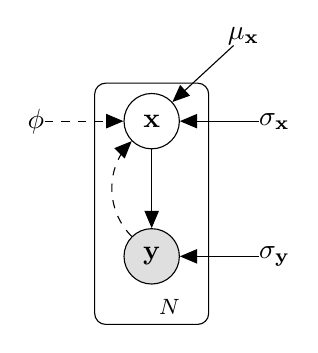
\begin{tikzpicture}[scale=1, transform shape]
\node[obs] (y1) {$\mathbf{y}$};
\node[latent, above=of y1] (x1) {$\mathbf{x}$};
\node[const, left=of x1] (phi1) {$\phi$};
\node[const, above right=of x1] (mu_x) {$\mu_{\mathbf{x}}$};
\node[const, right=of x1] (sigma_x) {$\sigma_{\mathbf{x}}$};
\node[const, right=of y1] (sigma_y) {$\sigma_{\mathbf{y}}$};
\edge [dashed] {phi1} {x1};
\edge {mu_x} {x1};
\edge {sigma_x} {x1};
\edge {sigma_y} {y1};
\draw (y1) edge[out=135,in=225,->,dashed] (x1);
\edge {x1} {y1};
\plate [xscale=1.5] {} {(y1)(x1)} {$N$} ;
\end{tikzpicture}
\end{flushright}
\end{minipage}
\end{minipage}

% Discrete
\begin{minipage}{\linewidth}
\begin{minipage}{0.66\linewidth}
\begin{lstlisting}[style=smaller]
var obs = loadData('data.json');
var nComps = 3;
var guideNet = nn.mlp(1, [{nOut: 3, activation: nn.sigmoid}, {nOut: nComps-1}], 'guideNet');
var model = function() {
   var theta_x = simplex(paramVector(nComps-1, 'theta_x'));
   var params_y = [
      {mu: paramScalar('mu_y_1'), sigma: softplus(paramScalar('sigma_y_1'))},
      {mu: paramScalar('mu_y_2'), sigma: softplus(paramScalar('sigma_y_2'))},
      {mu: paramScalar('mu_y_3'), sigma: softplus(paramScalar('sigma_y_3'))}
   ];
   var latents = mapData({data: obs}, function(y) {
      var nnInput = Vector([y]);
      var nnOutput = nnEval(guideNet, nnInput);
      var x = sample(Discrete({ps: theta_x}), {
         guide: Discrete(simplex(nnOutput))
      });
      observe(Gaussian(params_y[x]), y);
      return {x: x};
   });
   return latents;
};
\end{lstlisting}
\end{minipage}
%
\begin{minipage}{0.33\linewidth}
\begin{flushright}
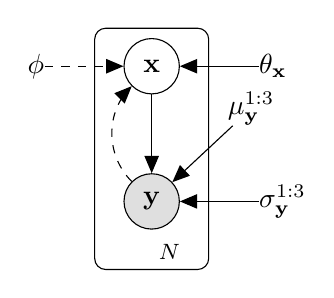
\begin{tikzpicture}[scale=1, transform shape]
\node[obs] (y1) {$\mathbf{y}$};
\node[latent, above=of y1] (x1) {$\mathbf{x}$};
\node[const, left=of x1] (phi1) {$\phi$};
\node[const, right=of x1] (theta_x) {$\theta_{\mathbf{x}}$};
\node[const, above right=of y1] (mu_y) {$\mu^{1\colon3}_{\mathbf{y}}$};
\node[const, right=of y1] (sigma_y) {$\sigma^{1\colon3}_{\mathbf{y}}$};
\edge [dashed] {phi1} {x1};
\edge {theta_x} {x1};
\edge {mu_y} {y1};
\edge {sigma_y} {y1};
\draw (y1) edge[out=135,in=225,->,dashed] (x1);
\edge {x1} {y1};
\plate [xscale=1.5] {} {(y1)(x1)} {$N$} ;
\end{tikzpicture}
\end{flushright}
\end{minipage}
\end{minipage}

\caption{WebPPL code and corresponding graphical models for simple Bayesian networks with one latent variable per observation. \emph{Top:} Continuous latent variable. \emph{Bottom:} Discrete latent variable with 3 discrete values (i.e. a Gaussian mixture model with 3 mixture components).}
\label{fig:bn_oneLatent}

\end{figure}


Figure~\ref{fig:bn_twoLatent} Top shows a slightly more complex Bayesian network with two latent continuous variables. Note that the guide program in this example predicts the two latent variables independently given the observation $\vecstyle{y}$. In Figure~\ref{fig:bn_twoLatent} Bottom, we make some small changes to the code (lines 3 and 17, highlighted in green) to instead have the guide program predict the second latent variable $\vecstyle{x}_2$ as a function of the first latent variable $\vecstyle{x}_1$. This small change allows the guide to capture a posterior dependency that was ingored by the first version.
\remark{We'll show later how this gives better results?}


\begin{figure}

% Two continuous; independent
\begin{minipage}{\linewidth}
\begin{minipage}{0.66\linewidth}
\begin{lstlisting}[style=smaller]
var obs = loadData('data.json');
var guideNet1 = nn.mlp(1, [{nOut: 3, activation: nn.sigmoid}, {nOut: 2}], 'guideNet1');
var guideNet2 = nn.mlp(1, [{nOut: 3, activation: nn.sigmoid}, {nOut: 2}], 'guideNet2');
var model = function() {
   var mu_x1 = paramScalar('mu_x1');
   var sigma_x1 = softplus(paramScalar('sigma_x1'));
   var mu_x2 = paramScalar('mu_x2');
   var sigma_x2 = softplus(paramScalar('sigma_x2'));
   var sigma_y = softplus(paramScalar('sigma_y'));
   var latents = mapData({data: obs}, function(y) {
      var nnInput1 = Vector([y]);
      var nnOutput1 = nnEval(guideNet1, nnInput1);
      var x1 = sample(Gaussian({mu: mu_x1, sigma: sigma_x1}), {
         guide: Gaussian({mu: T.get(nnOutput1, 0),
                          sigma: softplus(T.get(nnOutput1, 1))})
      });
      var nnInput2 = Vector([y]);
      var nnOutput2 = nnEval(guideNet2, nnInput2);
      var x2 = sample(Gaussian({mu: mu_x2, sigma: sigma_x2}), {
         guide: Gaussian({mu: T.get(nnOutput2, 0),
                          sigma: softplus(T.get(nnOutput2, 1))})
      });
      observe(Gaussian({mu: x1 + x2, sigma: sigma_y}), y);
      return {x1: x1, x2: x2};
   });
   return latents;
};
\end{lstlisting}
\end{minipage}
%
\begin{minipage}{0.33\linewidth}
\begin{flushright}
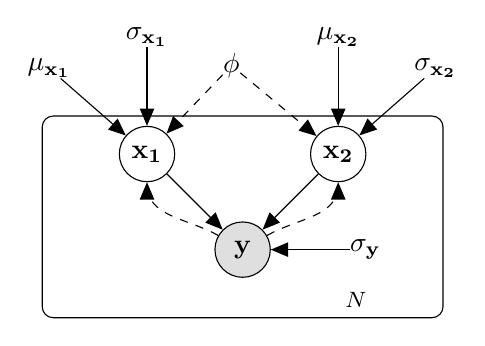
\begin{tikzpicture}[scale=1, transform shape]
\node[obs] (y1) {$\mathbf{y}$};
\node[latent, above left=of y1] (x1) {$\mathbf{x_1}$};
\node[latent, above right=of y1] (x2) {$\mathbf{x_2}$};
\node[const, above right=of x1] (phi1) {$\phi$};
\node[const, above left=of x1] (mu_x1) {$\mu_{\mathbf{x_1}}$};
\node[const, above=of x1] (sigma_x1) {$\sigma_{\mathbf{x_1}}$};
\node[const, above=of x2] (mu_x2) {$\mu_{\mathbf{x_2}}$};
\node[const, above right=of x2] (sigma_x2) {$\sigma_{\mathbf{x_2}}$};
\node[const, right=of y1] (sigma_y) {$\sigma_{\mathbf{y}}$};
\edge [dashed] {phi1} {x1};
\edge [dashed] {phi1} {x2};
\edge {mu_x1} {x1};
\edge {sigma_x1} {x1};
\edge {mu_x2} {x2};
\edge {sigma_x2} {x2};
\edge {sigma_y} {y1};
\draw (y1) edge[out=150,in=270,->,dashed] (x1);
\draw (y1) edge[out=30,in=270,->,dashed] (x2);
\edge {x1} {y1};
\edge {x2} {y1};
\plate [xscale=1.5] {} {(y1)(x1)(x2)} {$N$} ;
\end{tikzpicture}
\end{flushright}
\end{minipage}
\end{minipage}

% Two continuous; dependent
\begin{minipage}{\linewidth}
\begin{minipage}{0.66\linewidth}
\begin{lstlisting}[style=smaller]
var obs = loadData('data.json');
var guideNet1 = nn.mlp(1, [{nOut: 3, activation: nn.sigmoid}, {nOut: 2}], 'guideNet1');
var guideNet2 = nn.mlp(<@\hilite{2}@>, [{nOut: 3, activation: nn.sigmoid}, {nOut: 2}], 'guideNet2');
var model = function() {
   var mu_x1 = paramScalar('mu_x1');
   var sigma_x1 = softplus(paramScalar('sigma_x1'));
   var mu_x2 = paramScalar('mu_x2');
   var sigma_x2 = softplus(paramScalar('sigma_x2'));
   var sigma_y = softplus(paramScalar('sigma_y'));
   var latents = mapData({data: obs}, function(y) {
      var nnInput1 = Vector([y]);
      var nnOutput1 = nnEval(guideNet1, nnInput1);
      var x1 = sample(Gaussian({mu: mu_x1, sigma: sigma_x1}), {
         guide: Gaussian({mu: T.get(nnOutput1, 0),
                          sigma: softplus(T.get(nnOutput1, 1))})
      });
      var nnInput2 = <@\hilite{Vector([y, x1]);}@>
      var nnOutput2 = nnEval(guideNet2, nnInput2);
      var x2 = sample(Gaussian({mu: mu_x2, sigma: sigma_x2}), {
         guide: Gaussian({mu: T.get(nnOutput2, 0),
                          sigma: softplus(T.get(nnOutput2, 1))})
      });
      observe(Gaussian({mu: x1 + x2, sigma: sigma_y}), y);
      return {x1: x1, x2: x2};
   });
   return latents;
};
\end{lstlisting}
\end{minipage}
%
\begin{minipage}{0.33\linewidth}
\begin{flushright}
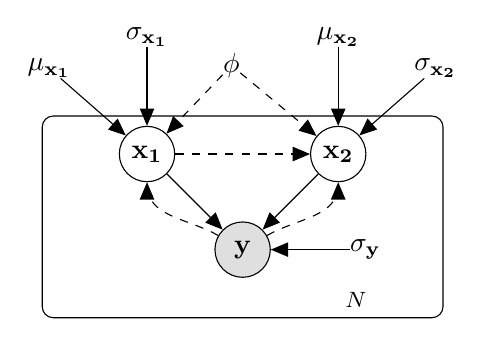
\begin{tikzpicture}[scale=1, transform shape]
\node[obs] (y1) {$\mathbf{y}$};
\node[latent, above left=of y1] (x1) {$\mathbf{x_1}$};
\node[latent, above right=of y1] (x2) {$\mathbf{x_2}$};
\node[const, above right=of x1] (phi1) {$\phi$};
\node[const, above left=of x1] (mu_x1) {$\mu_{\mathbf{x_1}}$};
\node[const, above=of x1] (sigma_x1) {$\sigma_{\mathbf{x_1}}$};
\node[const, above=of x2] (mu_x2) {$\mu_{\mathbf{x_2}}$};
\node[const, above right=of x2] (sigma_x2) {$\sigma_{\mathbf{x_2}}$};
\node[const, right=of y1] (sigma_y) {$\sigma_{\mathbf{y}}$};
\edge [dashed] {phi1} {x1};
\edge [dashed] {phi1} {x2};
\edge {mu_x1} {x1};
\edge {sigma_x1} {x1};
\edge {mu_x2} {x2};
\edge {sigma_x2} {x2};
\edge {sigma_y} {y1};
\draw (y1) edge[out=150,in=270,->,dashed] (x1);
\draw (y1) edge[out=30,in=270,->,dashed] (x2);
\edge [dashed] {x1} {x2};
\edge {x1} {y1};
\edge {x2} {y1};
\plate [xscale=1.5] {} {(y1)(x1)(x2)} {$N$} ;
\end{tikzpicture}
\end{flushright}
\end{minipage}
\end{minipage}

\caption{WebPPL code and corresponding graphical models for simple Bayesian networks with two latent variables per observation. \emph{Top:} Guide program predicts the two latents independently. \emph{Bottom:} Changing the guide program to treat the second latent variable as conditional on the first (green highlights show changes to the code).}
\label{fig:bn_twoLatent}
\end{figure}



%auto-ignore
\section{Optimizing Parameters}
\label{sec:optimization}

Now that we have seen how to author learnable guide programs, in this section, we will describe how to optimize the parameters of those programs. 

\subsection{Optimization Interface}

In Section~\ref{sec:pplbasics}, we showed how WebPPL programs use the \ic{Infer} function to perform non-amortized inference on a \ic{model} function. To optimize parameters for amortized inference, WebPPL provides an \ic{Optimize} function with a similar interface:
%%%
\begin{lstlisting}
var model = function() {
   // Use sample, guide, mapData, etc.
};

var params = Optimize(model, {
   steps: 100,
   optMethod: 'adam'
});
\end{lstlisting}
%%%
The code above performs 100 gradient update steps on \ic{model} using the Adam stochastic optimization method~\cite{Adam}.
The return value \ic{params} of this function is a map from parameter names to optimized parameter values. Section~\ref{sec:usingLearnedGuides} describes how to use these optimized parameters for inference tasks.

The remainder of this section focuses on the theory and implementation of our gradient-based optimization system. 

\subsection{ELBo: The Variational Objective}

In Section~\ref{sec:background:variational}, we mentioned that the goal of variational inference is to find values of the parameters $\phi$ for our guide program $\guidePosterior$ such that it is as close as possible to the true posterior $\truePosterior$, where closeness is measured via KL-divergence. The KL-divergence between two general distributions is intractable to compute; however, some straightforward algebra produces an objective that is tractable:
%%%
\begin{align}
\begin{split}
\KLD(\guidePosterior || \truePosterior)
&= \int_{\latentVars} \guidePosterior \log \frac{\guide(\guidePosterior}{\truePosterior}\\
&= \int_{\latentVars} \guidePosterior \log \frac{\guidePosterior}{\trueJoint} + \log \dataMarginal\\
&= \expect_{\guide}[ \log(\guidePosterior -  \trueJoint ) ] + \log \dataMarginal\\
&= \log \dataMarginal - \elboDef\\
&= \log \dataMarginal - \elbo \geq 0
\end{split}
\label{eq:elbo}
\end{align}
%%%
where the last inequality follows because KL-divergence is non-negative. This in turn implies that $\elbo$ is a lower bound on the log marginal likelihood of the data (i.e. evidence) $\log \dataMarginal$. Accordingly, $\elbo$ is sometimes referred to as the `Evidence Lower Bound', or ELBo~\cite{BBVI}. Maximizing the ELBo corresponds to minimizing the KL-divergence.
\remark{More generally (when logp(y) is an arbitrary partition function) this is the `variational free energy'.}

When learning a generative model $\trueJointTheta$, the objective is usually to maximize the log marginal likelihood of the training data $\log \dataMarginalTheta$. Rewriting the result from Equation~\ref{eq:elbo}:
%%%
\begin{equation*}
\elboWithTheta = \log \dataMarginalTheta - \KLD(\guidePosterior || \truePosteriorTheta)
\end{equation*}
%%%
we can see that, again, because KL-divergence is non-negative, maximizing the ELBo also corresponds to maximizing the log marginal likelihood of the data. Thus, whether we are doing amortized infernence only or amortized inference plus model learning, we can use the same optimization objective: the ELBo.

For an alternative derivation of the ELBo using Jensen's inequality, see Mnih and Gregor~\cite{NVIL} and Jordan et al.~\cite[p. 213]{VariationalInference}.

\subsection{ELBo Gradient Estimators}

Maximizing the ELBo requires estimating its gradient with respect to the parameters. For model learning, computing the gradient with respect to the model parameters $\theta$ is straightforward:
%%%
\begin{align}
\begin{split}
\gradparamsTheta \elboWithTheta
&= \gradparamsTheta \elboDefGenTheta\\
&= \expect_\guide [ \gradparamsTheta \log \trueJointTheta ] 
\end{split}
\label{eq:modelParamGrad}
\end{align}
%%%
where the expectation with respect to $\guide$ is approximated by samples drawn from $\guide$. This requires that $\trueJointTheta$ be differentiable with respect to $\theta$; many generative models with differentiable likelihoods have this property.

Estimating the gradient with respect to the guide parameters $\phi$ is more complex.
There are two well-known approaches to performing this estimation:

\paragraph{Likelihood Ratio (LR) Estimator:}
In the general case, the gradient of the ELBo with respect to $\phi$ can be estimated by:
%%%
\begin{align}
\begin{split}
\gradparams \elboWithTheta
&= \gradparams \elboDefGenTheta\\
&= \expect_\guide[ \gradparams \log \guidePosterior ( \log \trueJointTheta - \log \guidePosterior ) ]
\end{split}
\label{eq:lr}
\end{align}
%%%
This estimator goes by the names `likelihood ratio estimator'~\cite{LikelihoodRatioEstimator} and `score function estimator'~\cite{ScoreFunctionEstimator}, and it is also equivalent to the REINFORCE policy gradient algorithm in the reinforcement learning literature~\cite{REINFORCE}. The derivations of this estimator most relevant to our setting can be found in Wingate and Weber~\cite{AVIPP} and Mnih and Gregor~\cite{NVIL}.
Intuitively, each gradient update step using the LR estimator pushes the parameters $\phi$ in the direction $( \log \trueJoint - \log \guidePosterior )$---that is, the direction that will bring the guide closer to the true posterior. The magnitude of this update is controlled by $\gradparams \log \guidePosterior$.

The LR estimator is straightforward to compute, requiring only that $\log \guidePosterior$ be differentiable with respect to $\phi$ (the mean field and neural guide families presented in Section~\ref{sec:background} satisfy this property). However, it is known to exhibit high variance. This problem is amenable to several variance reduction techniques, some of which we will employ later in this section.

\paragraph{Pathwise (PW) Estimator:}

Equation~\ref{eq:lr} is more complicated (and less well-behaved) than Equation~\ref{eq:modelParamGrad} because the gradient can no longer be pushed inside the expectation: the expectation is with respect to $\guide$, and $\guide$ depends on the parameters $\phi$ with respect to which we are differentiating.
However, in certain cases, it is possible to re-write the ELBo such that the expectation distribution does not depend on $\phi$.
This situation occurs whenever the latent variables $\latentVars$ can be expressed as samples from an un-parameterized distribution, followed by a parameterized deterministic transformation:
%%%
\begin{equation*}
\latentVars = \xformedVarsPhi \hspace{2em} \reparamVars \sim \reparamDist(\cdot)
\end{equation*}
%%%
For example, sampling from a (multivariate) Gaussian distribution $\normdist(\mu, \Sigma)$ can be expressed as $\mu + \Sigma \cdot \reparamVars$, where $\reparamVars \sim \normdist(0, I)$. Continuous random variables which are parameterized by a location and a scale parameter naturally support this type of transformation, and other types of continuous variables can be well-approximated by deterministic transformations of uniform or unit normal variables~\cite{ADVI}.

Using this `reparameterization trick'~\cite{AEVB} allows the ELBo gradient to be rewritten as:
%%%
\begin{align}
\begin{split}
\gradparams \elboWithTheta
&= \gradparams \elboDefGenTheta\\
&= \gradparams \expect_\reparamDist [ \log p(\xformedVarsPhi, \observedVars ; \theta) - \log \guide(\xformedVarsPhi | \observedVars ; \phi) ]\\
&= \expect_\reparamDist [\gradparams ( \log p(\xformedVarsPhi, \observedVars ; \theta) - \log \guide(\xformedVarsPhi | \observedVars ; \phi) ) ]
\end{split}
\label{eq:pw}
\end{align}
%%%
This estimator is called the `pathwise derivative estimator'~\cite{PathwiseEstimator}.
It transforms both the guide and target distributions into distributions over independent random `noise' variables $\reparamVars$, followed by complex, parameterized, deterministic transformations. Given a fixed assignment to the noise variables, derivatives can propagate from the final log probabilities back to the input parameters, leading to much more stable gradient estimates than with the LR estimator.

\subsection{Hybrid Gradient Estimator for Guide Programs}

To make things as simple as possible, going to roll everything into one esimator. Use just $\phi$ for both generative and guide params, b/c it simplifies notation and reflects the fact that our system makes no distinction under the hood.

Hybrid PW/LR estimator. Each term drops out in certain conditions (refer to appendix for proofs). How our AD implementation handles this dropping out implicitly.

Cite stochastic computation graphs paper.

Argue that this deals properly with open worlds (ie can ignore rvs / params that weren’t touched on a given sample from q). Only (lazily) create parameter when you first hit it, only update it when RVs that it depend on are hit. Need lemma: gradient for param is zero if none of the RV’s it flows into are hit during a run. Again, with our AD, you don’t have to do any special cases to deal with this, it just falls out naturally.

Variance reduction for LR part of estimator. Dependence graph to eliminate weight contributions from RVs which are upstream in the dataflow graph (refer to appendix for proof) (cite inspiration from Rao-Blackwellization in other papers). mapData as a special case of this (but refer to appendix for its own proof?) Baselines (cite original papers that used it)---proof of correctness is short enough that we can just have it inline?



%auto-ignore
\section{Using Learned Parameters}
\label{sec:usingLearnedGuides}

Given a set of learned parameters, our system can predict latent variables, generate synthetic data, or further refine parameters for a new dataset or a new model.

\subsection{Predicting Latent Variables}

A learned guide can be used to make inferences about new, never-before-seen observations. As an example, we'll use the Gaussian mixture model program in Figure~\ref{fig:bn_oneLatent} Bottom and show how to predict cluster assignments for new observations. Note that the observations used by the program are assigned to the \ic{obs} variable, which is then passed to \ic{mapData}. WebPPL is a purely functional language, so it does not support assigning a new dataset to \ic{obs}. However, it does provide a special \ic{globalStore} object whose fields can be re-assigned. With this in mind, we modify the Gaussian mixture model program as follows\footnote{An alternative to using \ic{globalStore} for mutation would be to re-create the \ic{model} function, closing over the test data instead of the training data.}:
%%%
\begin{lstlisting}
globalStore.data = loadData('data.json');
// Set up guide neural net
var model = function() {
   // Set up generative parameters
   var latents = mapData({data: globalStore.data}, function(y) {
      // Guided sample latents, observe data points
   });
   return latents;
};
\end{lstlisting}
%%%
Now we can easily swap datasets using \ic{globalStore.data}. Given a set of learned parameters \ic{params} for this program, we can obtain a sample prediction for the latent variables for a new dataset:
%%%
\begin{lstlisting}
globalStore.data = loadData('data_test.json');	// Load new test data set

// Forward sample from the guide
sample(Infer({method: 'forward', guide: true, params: params}, model));

// Use the guide as a Sequential Monte Carlo importance sampler
sample(Infer({method: 'SMC', particles: 100, params: params}, model));
\end{lstlisting}
%%%
We can make predictions either by running the guide program forward, or if the true posterior is very complex and the learned guide only partially approximates it, we can use the guide program as an importance sampler within Sequential Monte Carlo.

\subsection{Generating Synthetic Data}

Forward sampling from the guide can also be used to generate synthetic data from the learned distribution. If we make a slightly modified version of the Gaussian mixture model (call it \ic{modelGen}) that samples data instead of observing it, we can used forward sampling with the optimized parameters \ic{params} to synthesize new data points:
%%%
\begin{lstlisting}
var modelGen = function() {
   var theta_x = simplex(modelParam({dims: [nComps-1, 1], name: 'theta_x'}));
   var params_y = [
      {mu: modelParam({name: 'mu1'}), sigma: softplus(modelParam({name: 's1'}))},
      {mu: modelParam({name: 'mu2'}), sigma: softplus(modelParam({name: 's2'}))},
      {mu: modelParam({name: 'mu3'}), sigma: softplus(modelParam({name: 's3'}))}
   ];
   var x = sample(Discrete({ps: theta_x}));
   return sample(Gaussian(params_y[x]));
};

sample(Infer({method: 'forward', guide: true, params: params}, modelGen));
\end{lstlisting}

\subsection{Further Optimization}
\label{sec:furtherOptim}

A set of learned parameters \ic{params} can also be passed back into \ic{Optimize} for further optimization:
%%%
\begin{lstlisting}
var newParams = Optimize(model, {
   steps: 100,
   optMethod: 'adam',
   params: params
});
\end{lstlisting}
%%%
This can be useful for e.g. fine-tuning existing parameters for a new dataset. Indeed, \ic{model} does not even need to be the same program that was originally used to learn \ic{params}; it just needs to declare some parameters (via \ic{param}) with the same names as parameters in \ic{params}. This can be useful for, for example, making a modification to an existing model without having to re-train its guide program from scratch, or for bootstrap training from a simpler model to a more complex one.


%auto-ignore
\section{Experiments}
\label{sec:results}

Having detailed how to specify and optimize guide programs in our system, in this section, we experimentally evaluate how well programs written in our system can learn generative models and approximate posterior samplers. Unless stated otherwise, we use the following settings for the experiments in this section:
%%%
\begin{itemize}
\item{The Adam optimization method~\cite{Adam} with $\alpha = 0.1$, $\beta_1 = 0.9$, and $\beta_2 = 0.99$.}
\item{One sample from $\guide$ per optimization step to estimate the expectation in Equation~\ref{eq:finalEstimator}.}
\end{itemize}

\subsection{Gaussian Mixture Model}
\label{sec:results_gmm}

We first consider the simple Gaussian mixture model program from Figure~\ref{fig:bn_oneLatent} Bottom. This program samples discrete random choices, so its gradient estimator will include an LR term. Alternatively, we could re-write the program slightly to explicitly marginalize out the discrete random choices; see Appendix~\ref{sec:appendix_code:gmmSumOut}. The gradient estimator for this program then reduces to the PW estimator, which will have lower variance. Lower variance comes at the cost of amortized inference, however, as this version of the program does not have a guide which can predict the latent cluster assignment given an observed point. We also consider a non-amortized, mean field version of the program for comparison.

Figure~\ref{fig:gmmResults} illustrates the performance of these programs after training for 200 steps on a synthetic datset of 100 points. On the left, we show how the ELBo changes during optimizaton. Even on a simple model such as this one, the ability to use the pure PW estimator leads to faster convergence and a better final objective score.
On the right, we show the estimated negative log likelihood of a separate synthetic test set under each program after optimization. Here, we also include the true model (i.e. the model used to synthesize the test/training data) for comparsion.
As suggested by its optimization performance, the model with discrete choices marginalized out performs best.
Note that the amortized guide program slightly out-performs the mean field guide program, indicating that the generalization provided by amortization has benefits for training generative models, in addition to enabling fast predictions of latent variables for previously-unseen observations.

\begin{figure}[!ht]
\begin{minipage}{0.5\linewidth}
\centering
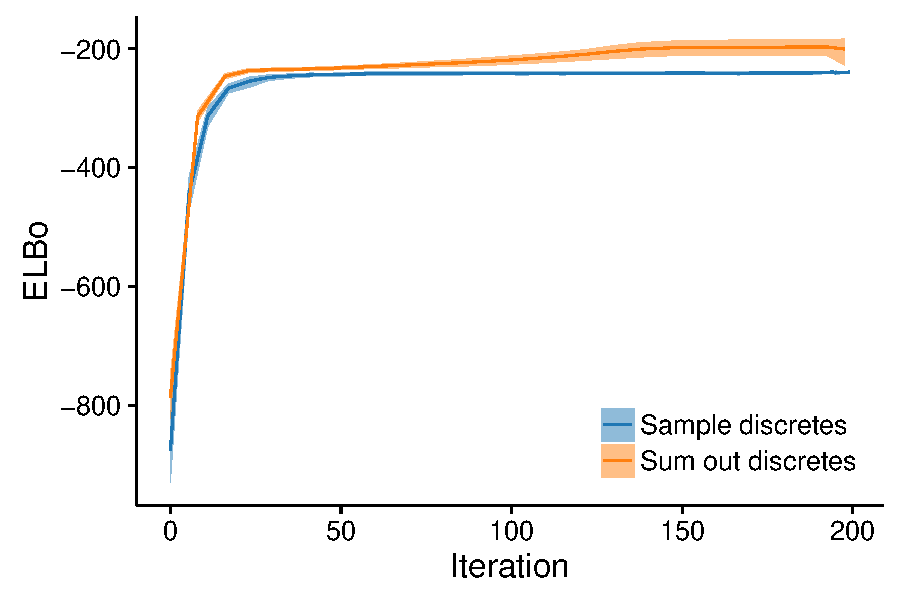
\includegraphics[width=\linewidth]{figs/results/gmm/elboProgress.pdf}
\end{minipage}
%
\begin{minipage}{0.5\linewidth}
\centering
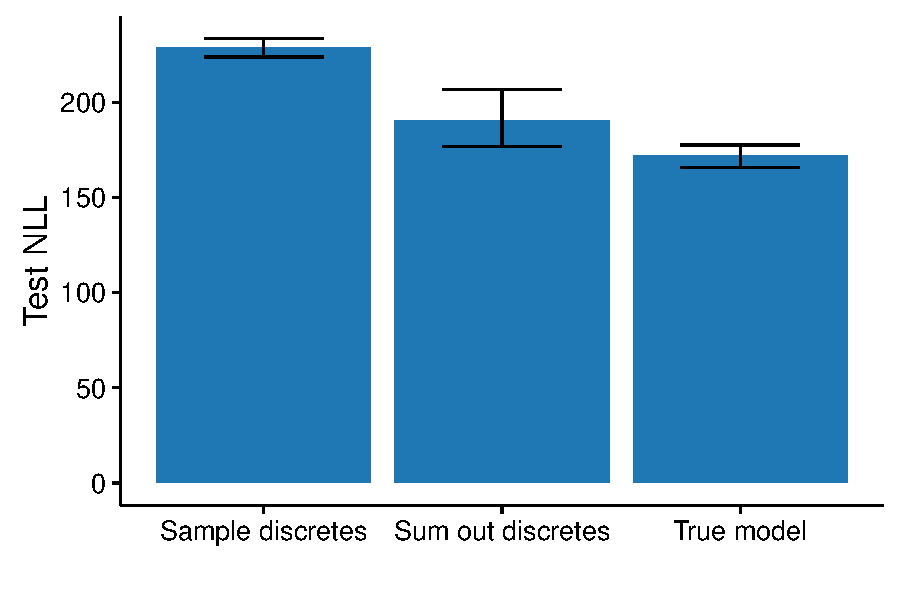
\includegraphics[width=\linewidth]{figs/results/gmm/nll.pdf}
\end{minipage}
\caption{Performance of simple Gaussian mixture model program. \emph{(Left)} ELBo optimization progress during training. \emph{(Right)} Negative log-likelihood of a held-out test set.}
\label{fig:gmmResults}
\end{figure}

% Other Bayes net examples??

\subsection{QMR-DT}
\label{sec:results_qmr}

We next consider a more complicated Bayesian network model based on the QMR-DT medical diagnosis network~\cite{QMR}. QMR-DT is a bipartite graphical model with one layer of nodes corresponding to latent causes (e.g. diseases, in the medical setting) and a second layer of observed effects (e.g. symptoms). All nodes are binary (i.e. Bernoulli), and the cause nodes are connected to the effects via directed noisy-or links. Appendix~\ref{sec:appendix_code:qmr} shows our implementation.

Our amortized guide program for this model uses a neural network to jointly predict the probabilities of all latent cause variables given a set of observed effects. Since the QMR-DT model contains a large number of discrete random variables, we expect the variance reduction strategies introduced in Section~\ref{sec:optimization:unifiedEstimator} to have significant effect.
Thus, we consider training this guide program with no variance reduction (\emph{Amortized}), with per-choice likelihood ratio weights, (\emph{+ local weights}), and with both per-choice weights and baselines (\emph{+ baselines}). As a point of reference, we also include a mean field model which uses all variance reduction strategies.
Data for our experiments is sampled from a randomly-generated graph with 200 causes and 100 effects. We sample 1000 observations for the training set and an additional 100 for a held-out test set.
\ndg{note that the fully-marginalized approach isn't really tractable anymore due to the size of the latent space?}

Figure~\ref{fig:qmrResults} shows the results of our experiments. The left plot shows optimization progress under each condition. Without any of the variance reduction strategies, gradients are extremely noisy and optimization makes almost no progress. Using local, per-variable likelihood ratio weights allows optimization to mke progress, and adding per-variable baselines further boosts performance. Though it uses all variance reduction strategies, the mean field model trains significantly more slowly than the variance-reduced amortized models. This happens because the mean field model has separate parameters for each training observation, rather than a single parameter set shared by a neural network, i.e. it has many more parameters that are each updated by very few gradient steps. Amortization thus both facilitates fast posterior prediction and exhibits faster training due to parameter sharing.

We next evaluate the guide program's posterior prediction ability. We use the learned guide to sample latent causes given an observed set of effects from the test set, sample effects given those causes, and then record what percentage of active effects in the test set observation are correctly predicted by the effects `hallucinated' from our model. Specifically, if $\vecstyle{e}$ is a vector of effect variables of length $N$, then the metric we use is:
%%%
\begin{align*}
&\min(F(\vecstyle{e}_{\text{true}}, \vecstyle{e}_{\text{sampled}}), F(\vecstyle{e}_{\text{sampled}}, \vecstyle{e}_{\text{true}}))\\
&F(\vecstyle{e}_1, \vecstyle{e}_2) = \frac{1}{\sum_i^N \vecstyle{e}_1(i)} \sum_{i, \vecstyle{e}_1(i) = 1} \indicator{\vecstyle{e}_2(i) = 1}
\end{align*}
%%%
where $\vecstyle{e}_{\text{true}}$ are effects from the test set and $\vecstyle{e}_{\text{sampled}}$ are hallucinated from the model.
Figure~\ref{fig:qmrResults} Right plots the average $F$ score over 100 runs, where we compare our amortized guide program against using the prior program to sample latent causes. The learned guide program correctly predicts more than twice as many active effects.

\begin{figure}[!ht]
\begin{minipage}{0.6\linewidth}
\centering
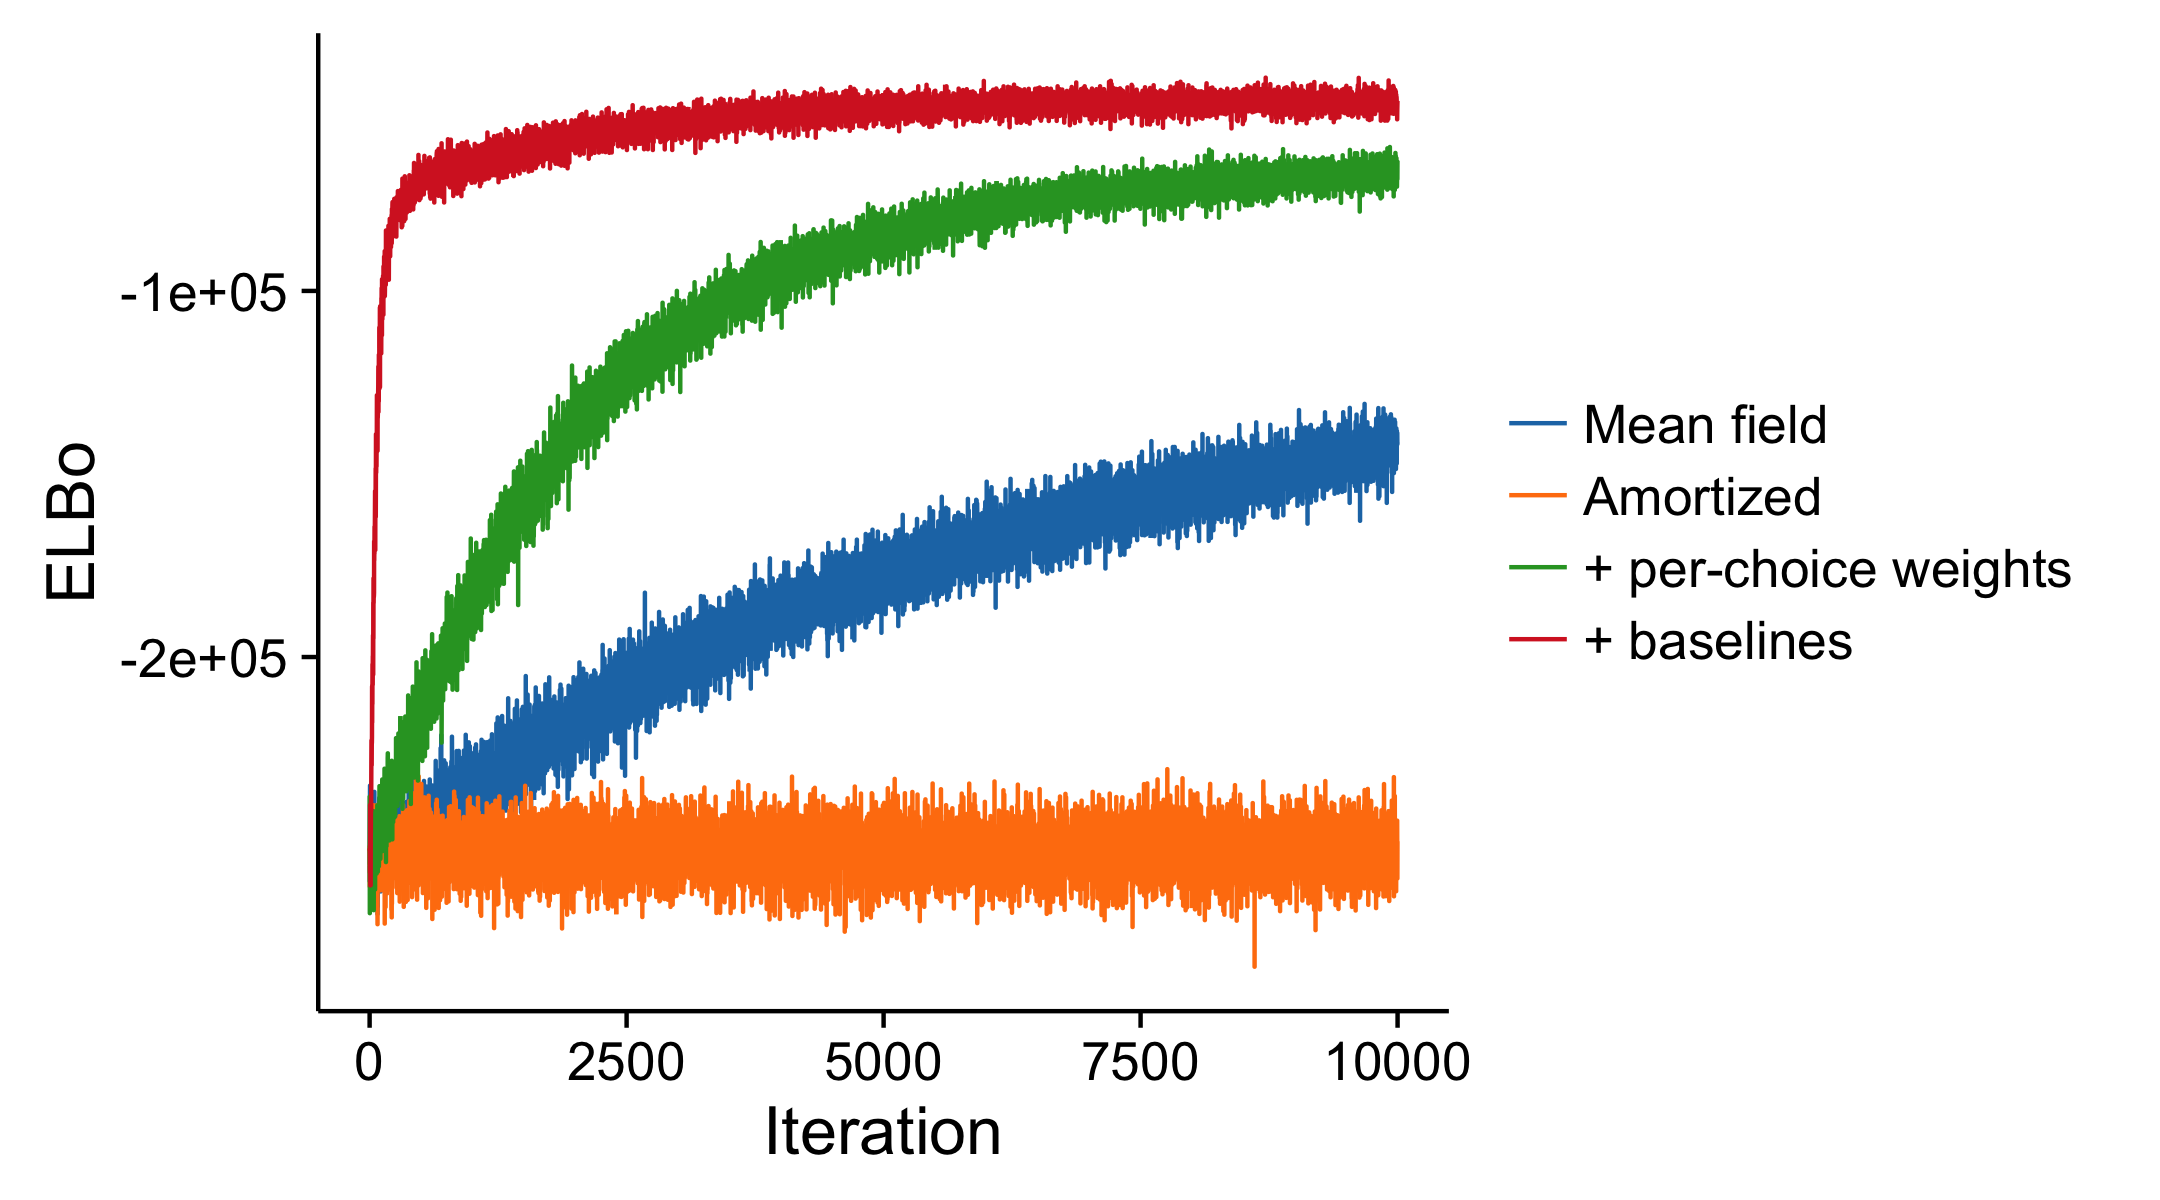
\includegraphics[width=\linewidth]{figs/results/qmr/elboProgress.png}
\end{minipage}
%
\begin{minipage}{0.4\linewidth}
\centering
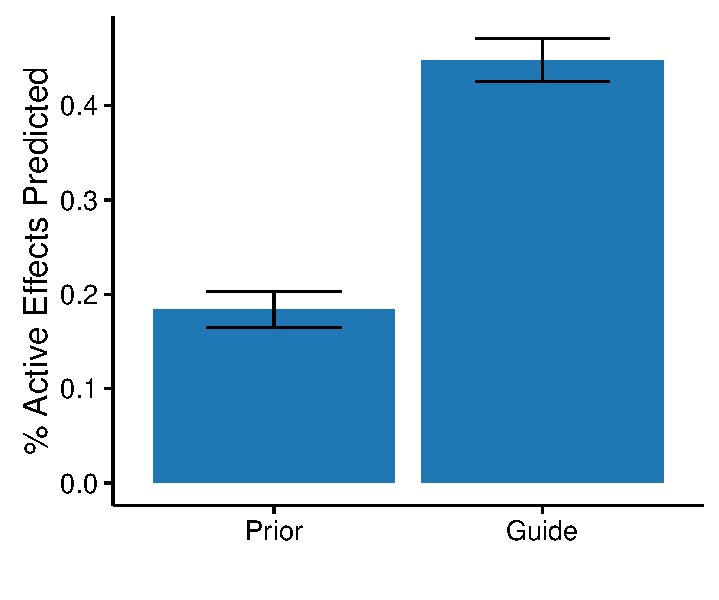
\includegraphics[width=\linewidth]{figs/results/qmr/reconstructScores.pdf}
\end{minipage}
\caption{Performance of a QMR-DT model. \emph{(Left)} ELBo optimization progress during training. \emph{(Right)} Percentage of test set active effects correctly predicted using latent causes sampled from either the prior or the guide program.}
\label{fig:qmrResults}
\end{figure}


\subsection{Neural Generative Models: Variational Autoencoder \& Sigmoid Belief Network}
\label{sec:results_vae}

Our system naturally supports generative models which use neural network components. Two prominent examples of models in this class include the Variational Autoencoder (VAE) and Sigmoid Belief Networks (SBN). Both models sample latent variables from a multivariate distribution and then transform the result via a neural network to produce observed variables, often in the form of an image. The VAE uses a latent multivariate Gaussian distribution, whereas the SBN uses a latent multivariate Bernoulli.

Appendix~\ref{sec:appendix_code} shows implementations of these models in our system. Our VAE implementation follows the original description of the model by Kingma and Welling~\cite{AEVB}, and our SBN implementation follows that of Mnih and Gregor~\cite{NVIL}.
The VAE uses a 20-dimensional latent code, and the SBN uses a single layer of 200 hidden variables. Our system cannot express the two-layer SBN of Mnih and Gregor, because its guide model samples the latent variables in the reverse order of the generative model.

Figure~\ref{fig:vae_sbn_results} Left shows results of training these models on the MNIST dataset, using Adam with a step size of 0.001.
While both models train quickly at first, the SBN's training slows more noticeably than the VAE's due to its discrete nature. It takes more than three times as many iterations to achieve the same ELBo.
In Figure~\ref{fig:vae_sbn_results} Right, we qualitatively evaluate both models by using them to reconstruct images from the MNIST test set. We use the guide program to sample latent variables conditional on the images in the ``Target'' column (i.e. the `encoder' phase). We then transform these latent variables using the generative model's neural networks (i.e. the `decoder' phase) to produce the reconstructed images in the ``VAE'' and ``SBN'' columns.
As suggested by their training behavior, the VAE is able to generate higher-quality reconstructions after less training.

Our optimization exhibits some differences from the previous work.
For the VAE, Kingma and Welling~\cite{AEVB} exploit the closed-form solution of the KL divergence between two Gaussians to create an even lower-variance estimator of the ELBo gradient. We use a more general formulation, but our system can still successfully train the model.
For the SBN, Mnih and Gregor~\cite{NVIL} use neural networks to compute the per-variable baselines $b_i$ in Equation~\ref{eq:finalEstimator}, whereas we use a simpler approach (see Appendix~\ref{sec:appendix_proofs}).
However, the key point is that each of these models was described in a simple WebPPL program with neural guides and optimized by the default system, without the need for additional implementation efforts.

\begin{figure}
\begin{minipage}{0.5\linewidth}
\centering
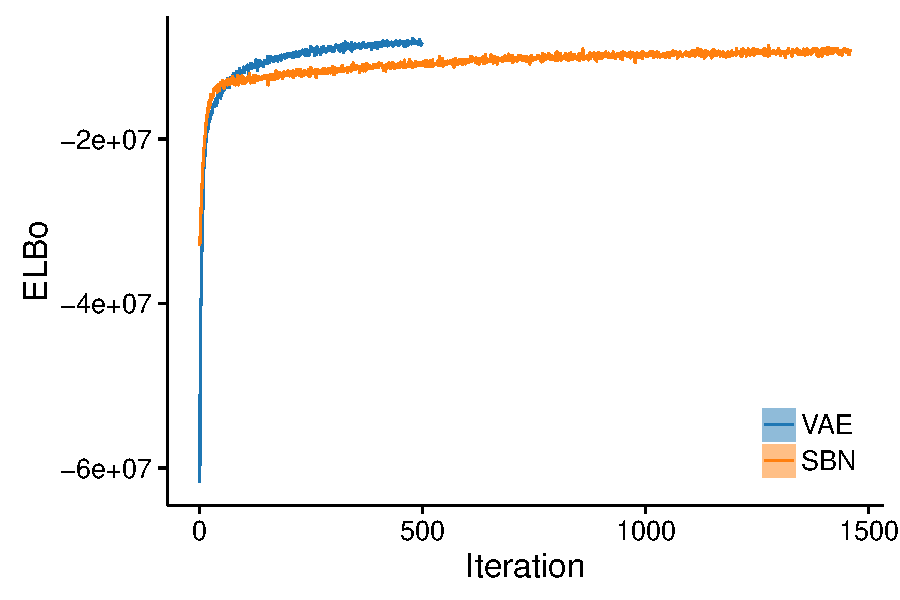
\includegraphics[width=\linewidth]{figs/results/vae_sbn/elboProgress.pdf}
\end{minipage}
%
\hspace{2em}
%
\begin{minipage}{0.5\linewidth}
\setlength{\tabcolsep}{1pt}
\centering
\begin{tabular}{c  c c c c c c}
Target & \multicolumn{3}{c}{VAE} & \multicolumn{3}{c}{SBN}
\\
 
\includegraphics[width=0.12\linewidth]{figs/results/vae_sbn/vae_encodeDecode_target_000.png}
 \hspace{3pt}
& 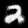
\includegraphics[width=0.12\linewidth]{figs/results/vae_sbn/vae_encodeDecode_target_000_sample_001.png}
& 
\includegraphics[width=0.12\linewidth]{figs/results/vae_sbn/vae_encodeDecode_target_000_sample_002.png}
& 
\includegraphics[width=0.12\linewidth]{figs/results/vae_sbn/vae_encodeDecode_target_000_sample_003.png}
\hspace{3pt}
& 
\includegraphics[width=0.12\linewidth]{figs/results/vae_sbn/sbn_encodeDecode_target_000_sample_001.png}
& 
\includegraphics[width=0.12\linewidth]{figs/results/vae_sbn/sbn_encodeDecode_target_000_sample_002.png}
& 
\includegraphics[width=0.12\linewidth]{figs/results/vae_sbn/sbn_encodeDecode_target_000_sample_003.png}
\\
 
\includegraphics[width=0.12\linewidth]{figs/results/vae_sbn/vae_encodeDecode_target_001.png}
 \hspace{3pt}
& 
\includegraphics[width=0.12\linewidth]{figs/results/vae_sbn/vae_encodeDecode_target_001_sample_001.png}
& 
\includegraphics[width=0.12\linewidth]{figs/results/vae_sbn/vae_encodeDecode_target_001_sample_002.png}
& 
\includegraphics[width=0.12\linewidth]{figs/results/vae_sbn/vae_encodeDecode_target_001_sample_003.png}
\hspace{3pt}
& 
\includegraphics[width=0.12\linewidth]{figs/results/vae_sbn/sbn_encodeDecode_target_001_sample_001.png}
& 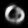
\includegraphics[width=0.12\linewidth]{figs/results/vae_sbn/sbn_encodeDecode_target_001_sample_002.png}
& 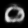
\includegraphics[width=0.12\linewidth]{figs/results/vae_sbn/sbn_encodeDecode_target_001_sample_003.png}
\\
 
\includegraphics[width=0.12\linewidth]{figs/results/vae_sbn/vae_encodeDecode_target_002.png}
 \hspace{3pt}
& 
\includegraphics[width=0.12\linewidth]{figs/results/vae_sbn/vae_encodeDecode_target_002_sample_001.png}
& 
\includegraphics[width=0.12\linewidth]{figs/results/vae_sbn/vae_encodeDecode_target_002_sample_002.png}
& 
\includegraphics[width=0.12\linewidth]{figs/results/vae_sbn/vae_encodeDecode_target_002_sample_003.png}
\hspace{3pt}
& 
\includegraphics[width=0.12\linewidth]{figs/results/vae_sbn/sbn_encodeDecode_target_002_sample_001.png}
& 
\includegraphics[width=0.12\linewidth]{figs/results/vae_sbn/sbn_encodeDecode_target_002_sample_002.png}
& 
\includegraphics[width=0.12\linewidth]{figs/results/vae_sbn/sbn_encodeDecode_target_002_sample_003.png}
\\
 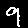
\includegraphics[width=0.12\linewidth]{figs/results/vae_sbn/vae_encodeDecode_target_003.png}
 \hspace{3pt}
& 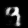
\includegraphics[width=0.12\linewidth]{figs/results/vae_sbn/vae_encodeDecode_target_003_sample_001.png}
& 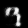
\includegraphics[width=0.12\linewidth]{figs/results/vae_sbn/vae_encodeDecode_target_003_sample_002.png}
& 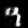
\includegraphics[width=0.12\linewidth]{figs/results/vae_sbn/vae_encodeDecode_target_003_sample_003.png}
\hspace{3pt}
& 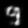
\includegraphics[width=0.12\linewidth]{figs/results/vae_sbn/sbn_encodeDecode_target_003_sample_001.png}
& 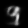
\includegraphics[width=0.12\linewidth]{figs/results/vae_sbn/sbn_encodeDecode_target_003_sample_002.png}
& 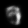
\includegraphics[width=0.12\linewidth]{figs/results/vae_sbn/sbn_encodeDecode_target_003_sample_003.png}
\end{tabular}
\end{minipage}
\caption{Evaluating the Variational Autoencoder (VAE) and Sigmoid Belief Network (SBN) programs on the MNIST dataset. \emph{(Left)} ELBo optimization progress during training. \emph{(Right)} Reconstructing the images in the ``Target'' column using both models.}
\label{fig:vae_sbn_results}
\end{figure}


\subsection{Latent Dirichlet Allocation}
\label{sec:results_lda}

Introduce the CoCoLab abstracts dataset (no citation, but acknowledge robert in footnote)

Do mean-field, marginalized, and one or two neural guides?

Show Top N words for each learned topic?


%Things to try if we have time:
%\begin{itemize}
%\item{Simple bayesian NN (show how easy it is to do full variational Bayes)}
%\item{HMM-type families: Deep kalman filter? Or other RNN VAE type thing?}
%\item{PCFG (prob won’t work, but useful to understand). Continuous feature-passing version?}
%\end{itemize}
%


%auto-ignore
\section{Deriving Guides Automatically}
\label{sec:autoGuide}

Thus far, we have shown how we can succesfully create and train guide programs for several types of generative models. However, writing guide programs can sometimes be tedious and repetitive; for example, note the large amount of shared structure between the guides shown in Figures~\ref{fig:bn_oneLatent} and \ref{fig:bn_twoLatent}. Furthermore, it is not always obvious how to write a good guide program. In Figure~\ref{fig:bn_twoLatent}, knowledge of the structure of this very simple generative model led us to add a direct dependency between the two latent variables in the guide. For general programs---especially large, complex ones---it will not always be clear what these dependencies are or how to capture them with a guide.

This section describes our early experience with automatically deriving guide programs. We first describe how our system provides sensible default behavior that can make writing some guides less cumbersome. We then outline how the system might be extended to automatically derive guides for any program using recurrent neural networks.

\subsection{Mean Field by Default}

If a call to \ic{sample} is not provided with an explicit guide distribution, our system automatically inserts a mean field guide. For example, the code \ic{sample(Gaussian(\{mu: 0, sigma: 1\}))} results in:
%%%
\begin{lstlisting}
sample(Gaussian({mu: 0, sigma: 1}), {
   guide: Gaussian({mu: paramScalar(<@\hilite{<auto_name>}@>), sigma: softplus(paramScalar(<@\hilite{<auto_name>}@>))})
})
\end{lstlisting}
%%%
where parameter bounding transforms such as \ic{softplus} are applied based on bounds metadata provided with each primitive distribution type. We use reparameterizable guides for continuous distributions (see Appendix~\ref{sec:appendix_reparam}).

Since this process declares new optimizable parameters automatically, we must automatically generate names for these parameters. Our system names parameters according to where they are declared in the program execution trace, using the same naming technique as is used for random choices in probabilistic programming MCMC engines~\cite{Lightweight}. Since the names of these parameters are tied to the structure of the program, they cannot be re-used by other programs (as in the `Further Optimization' example of Section~\ref{sec:furtherOptim}).

\subsection{Beyond Mean Field: Automatic Factored Guides with Recurrent Networks}

Call back to QMR factored guide results. Discuss how this might be generalized. Specifically, note that one can construct a guide like this for any program, because every program factors as a sequence of random choices. Rather than use a separate prediction network for each latent choice, use one prediction network with learnable address emdeddings. Mention that we are continuing experiments along these lines.

% \subsection{Capturing Posterior Dependencies with Context Nets}

% Context nets, val2vec, and vec2dist.

% When to init context (e.g. incorporating datum in each mapData iteration vs. something more global).

% Architecture choices: LSTM, bilinear resnets, linear predict net, etc.

% If we have time:
% \begin{itemize}
% \item{Context nets with long distance connections?}
% \item{Automatic mixtures for continuous distributions?}
% \item{Other interesting guides?}
% \end{itemize}




%auto-ignore
\section{Automatic Guide Experiments}
\label{sec:results_autoGuide}

Results for auto-guide stuff goes here.


\subsection{Latent Dirichlet Allocation Revisited}
\label{sec:results_autoGuide_lda}

Compare results of full auto guide to previous mean field version.


\subsection{QMR-DT}
\label{sec:results_autoGuide_qmr}

Make up a QMR model, compare mean field to auto guide with context net.


Additional experiments if time: some kind of time-series thing, e.g. Deep Kalman Filter?


%auto-ignore
\section{Conclusion}
\label{sec:conclusion}

Conclude, restate contributions. Discuss what we learned, etc.

\subsection{Future Work}
\label{sec:conclusion_futureWork}

Yield-so-far, accumulative models (cite NGPM).

More constructions like mapData. foldData?

More possibilities for auto-guide architectures: neural Turing machines (external memory might be better for capturing certain long-range dependencies), neural programmer-interpreter (the `stack' of recurrent networks, which communicate via arguments, might be a better representation for soe programs).

Tutorial training and combinations with SMC (also from NGPM), wakey-sleepy(?)

Variable re-ordering (i.e. the truly `backwards' model, cite stochastic inverse paper + Brooks's neural net version of stochastic inverses, NVIL 2-layer SBN). Including extra choices that don't hapen in the main program. Even more general control flow changes?


%auto-ignore

\section*{Acknowledgments}

This material is based on research sponsored by DARPA under agreement number FA8750-14-2-0009. The U.S. Government is authorized to reproduce and distribute reprints for Governmental purposes notwithstanding any copyright notation thereon. The views and conclusions contained herein are those of the authors and should not be interpreted as necessarily representing the official policies or endorsements, either expressed or implied, of DARPA or the U.S. Government.



% \small
\bibliographystyle{plain}
\bibliography{main}

\section{Appendix: Gradient Estimator Derivations \& Correctness Proofs}
\label{sec:appendix_proofs}

\newtheorem{lemma}{Lemma}
\newtheorem{theorem}{Theorem}

\subsection{Derivation of Unified Gradient Estimator (Equation~\ref{eq:hybridEstimator})}
\label{sec:appendix:estDerivation}

\begin{align}
\gradparams \elbo
%
&= \gradparams \expect_\reparamDist [ \log p(\xformedVars, \observedVars) - \log \guide(\xformedVars | \observedVars) ]\nonumber\\
%
&= \gradparams \int_\reparamVars \reparamDist(\reparamVars | \observedVars) ( \log p(\xformedVars, \observedVars) - \log \guide(\xformedVars | \observedVars) )\nonumber\\
%
&= \int_\reparamVars \gradparams \reparamDist(\reparamVars | \observedVars) ( \log p(\xformedVars, \observedVars) - \log \guide(\xformedVars | \observedVars) ) + \reparamDist(\reparamVars | \observedVars) \gradparams ( \log p(\xformedVars, \observedVars) - \log \guide(\xformedVars | \observedVars) )\nonumber \\
%
\label{eq:estDerivation_trick}
&= \int_\reparamVars \reparamDist(\reparamVars | \observedVars) \gradparams \log \reparamDist(\reparamVars | \observedVars) ( \log p(\xformedVars, \observedVars) - \log \guide(\xformedVars | \observedVars) ) + \reparamDist(\reparamVars | \observedVars) \gradparams ( \log p(\xformedVars, \observedVars) - \log \guide(\xformedVars | \observedVars) ) \\
%
&= \expect_\reparamDist [ \gradparams \log \reparamDist(\reparamVars | \observedVars) ( \log p(\xformedVars, \observedVars) - \log \guide(\xformedVars | \observedVars) ) + \gradparams( \log p(\xformedVars, \observedVars) - \log \guide(\xformedVars | \observedVars) )]\nonumber
\end{align}
Line~\ref{eq:estDerivation_trick} makes use of the identity $\nabla f(x) = f(x) \nabla \log f(x)$.

\subsection{Zero Expectation Identities}
\label{sec:appendix:zeroexp}

In what follows, we will make frequent use of the following:

\begin{lemma}
If $f(x)$ is a probability distribution, then:

\begin{equation*}
\expect_f[\nabla \log f(x)] = 0
\end{equation*}
\label{lem:zeroexp}
\end{lemma}
%%%
\begin{proof}
\begin{equation*}
\expect_f[\nabla \log f(x)]
%
= \int_x f(x) \nabla \log f(x)
%
= \int_x \nabla f(x)
%
= \nabla \int_x f(x)
%
= \nabla 1
%
= 0
\end{equation*}
\end{proof}

\begin{lemma}
For a discrete random choice $\reparamVar_i$ and a function $f(\reparamVars_{<i}, \observedVars)$:
%
\begin{equation*}
\expect_\reparamDist [ \gradparams \log \guide(\reparamXform_i(\reparamVar_i) | \reparamXform(\reparamVars_{<i}), \observedVars) f(\reparamVars_{<i}, \observedVars) ] = 0
\end{equation*}
\label{lem:zeroexp2}
\end{lemma}
%%%
\begin{proof}
\begin{align*}
\expect_\reparamDist [ \gradparams \log \guide(\reparamXform_i(\reparamVar_i) | \reparamXform(\reparamVars_{<i}), \observedVars) f(\reparamVars_{<i}, \observedVars) ]
%
&= \int_\reparamVars \reparamDist(\reparamVars | \observedVars) \gradparams \log \guide(\reparamXform_i(\reparamVar_i) | \reparamXform(\reparamVars_{<i}), \observedVars) f(\reparamVars_{<i}, \observedVars)\\
%
&= \int_\reparamVars \reparamDist(\reparamVars | \observedVars) \gradparams \log \reparamDist(\reparamVar_i | \reparamVars_{<i}, \observedVars) f(\reparamVars_{<i}, \observedVars)\\
%
&= \int_{\reparamVars_{<i}} \reparamDist(\reparamVars_{<i} | \observedVars) f(\reparamVars_{<i}, \observedVars) \sum_{\reparamVar_i} \reparamDist(\reparamVar_i | \reparamVars_{<i}, \observedVars) \gradparams \log \reparamDist(\reparamVar_i | \reparamVars_{<i}, \observedVars) \int_{\reparamVars_{>i}} \reparamDist(\reparamVars_{>i} | \reparamVars_{\leq i}, \observedVars)\\
%
&= \int_{\reparamVars_{<i}} \reparamDist(\reparamVars_{<i} | \observedVars) f(\reparamVars_{<i}, \observedVars) \cdot \expect_{\reparamDist} [ \gradparams \log \reparamDist(\reparamVar_i | \reparamVars_{<i}, \observedVars) ] \cdot 1\\
%
&= \int_{\reparamVars_{<i}} \reparamDist(\reparamVars_{<i} | \observedVars) f(\reparamVars_{<i}, \observedVars) \cdot 0 = 0
\end{align*}
where the last line makes use of Lemma~\ref{lem:zeroexp}.
\end{proof}

\subsection{Variance Reduction Step 1: Zero Expectation $W$ Terms}

In this section, we show that for each random choice $i$, we can remove terms from $W(\reparamVars, \observedVars)$ to produce $w_i(\reparamVars, \observedVars)$. Specifically, we prove that while $w_i(\reparamVars, \observedVars) \neq W(\reparamVars, \observedVars)$, we still have $\expect_\reparamDist [ \gradparams \log \guide(\reparamXform_i(\reparamVar_i) | \reparamXform(\reparamVars_{<i}), \observedVars) w_i(\reparamVars, \observedVars) ] = \expect_\reparamDist [ \gradparams \log \guide(\reparamXform_i(\reparamVar_i) | \reparamXform(\reparamVars_{<i}), \observedVars) W(\reparamVars, \observedVars) ]$.

To enable the computation of each $w_i$, our system builds a directed acyclic dependency graph as the program executes. The graph is constructed as follows:
%%%
\begin{itemize}
\item{\textbf{On program start:} Create a root node \ic{root}. Set \ic{prev = root}. This holds the previous node and will be used to assign node parents.}
\item{\textbf{On \ic{sample} or \ic{observe}:} Create a new node \ic{node} representing this random choice/observation. Set \ic{node.parent = prev}. Update \ic{prev = node}.}
\item{\textbf{On \ic{mapData} begin:} Create two new nodes \ic{split} and \ic{join}. These nodes will delimit the beginning and ending of the \ic{mapData} iteration. Push \ic{split, join} onto a stack \ic{mapDataStack}. This stack keeps track of \ic{split, join} nodes when there are nested calls to \ic{mapData}.}
\item{\textbf{On \ic{mapData} iteration begin:} Retrieve \ic{split, join = top(mapDataStack)}. Update \ic{prev = split}. This step reflects the independence assumptions of \ic{mapData}: an iteration of \ic{mapData} does not depend on any previous iterations, so there are no such edges in the graph. Instead, each iteration of \ic{mapData} points back to the beginning of the \ic{mapData} call.}
\item{\textbf{On \ic{mapData} iteration end:} Retrieve \ic{split, join = top(mapDataStack)}. Add \ic{prev} to \ic{join.parents}. This step connects the last random choice in each \ic{mapData} iteration to the \ic{join} node.}
\item{\textbf{On \ic{mapData} end:} Retrieve \ic{split, join = top(mapDataStack)}. Update \ic{prev = join}. This step acknowledges that any subsequent computation may depend on the \ic{mapData} as a whole.}
\end{itemize}
%%%
In this graph, all nodes correspond to random choices or observations, except for the special \ic{mapData} nodes \ic{split} and \ic{join}.
When there are no calls to \ic{mapData}, the graph has a linear topology, where each node is connected via a parent edge to the previously-sampled/observed node.
\ic{mapData} calls introduce fanout-fanin subgraphs: the \ic{split} node fans out into separate linear chains for each \ic{mapData} iteration, and the last nodes of these chains fan in to the \ic{join} node. Figure~\ref{fig:graphExample} shows the resulting graph for one execution of a simple example program.

\begin{figure}[!ht]
\begin{minipage}{0.65\linewidth}
\begin{lstlisting}
var data = loadData('data.json');
var model = function() {
   var a = sample(Bernoulli({p: 0.5}));
   mapData({data: data}, function(y) {
      var x = sample(Gaussian({mu: a ? 0 : 5, sigma: 1}));
      observe(Gaussian({mu: x, sigma: 0.5}), y);
   });
   return a;
}
\end{lstlisting}
\end{minipage}
%
\begin{minipage}{0.35\linewidth}
\centering
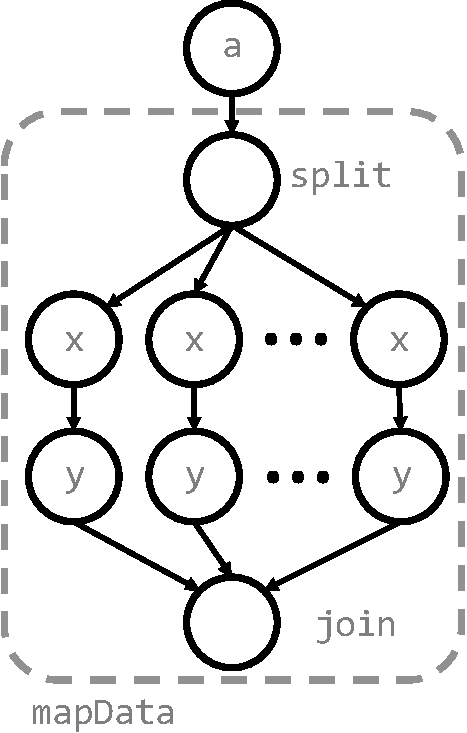
\includegraphics[width=\linewidth]{figs/graphExample.pdf}
\end{minipage}
\caption{A conservative dependency graph \emph{(Right)} resulting from one execution through a simple program \emph{(Left)}.}
\label{fig:graphExample}
\end{figure}

By construction, this graph is an overly-conservative dataflow dependency graph: if random choice $\reparamVar_a$ flows into random choice $\reparamVar_b$ (or observation $\observedVar_c$), then a path $\reparamVar_a \to \reparamVar_b$ (or $\reparamVar_a \to \observedVar_c$) exists in the graph. The converse is not necessarily true (i.e. there can exist edges between nodes that have no dataflow dependency). Note also that, by construction, the existence of a path $\reparamVar_a \to \reparamVar_b$ implies that $\reparamVar_b$ was sampled after $\reparamVar_a$ in the program execution order.

From the perpective of a random choice node $\reparamVar_i$, the graph nodes can be partitioned into the following subsets:
%%%
\begin{itemize}
\item{$\mathcal{D}_i$: the nodes ``downstream'' from $\reparamVar_i$ (i.e. the set of all nodes $d$ for which an edge $\reparamVar_i \to d$ exists.}
\item{$\mathcal{U}_i$: the nodes ``upstream'' from $\reparamVar_i$ (i.e the set of all nodes $u$ for which an edge $u \to \reparamVar_i$ exists.}
\item{$\mathcal{C}_i$: the set of nodes which are in neither $\mathcal{D}_i$ nor $\mathcal{U}_i$.}
\end{itemize}
%%%
Figure~\ref{fig:graphPartitions} illustrates these partitions on an example graph. For convenience, we also define $\mathcal{B}_i \equiv \mathcal{U}_i \cup \mathcal{C}_i$.

\begin{figure}[!ht]
\centering
%auto-ignore

%% Creator: Inkscape inkscape 0.91, www.inkscape.org
%% PDF/EPS/PS + LaTeX output extension by Johan Engelen, 2010
%% Accompanies image file 'graph.pdf' (pdf, eps, ps)
%%
%% To include the image in your LaTeX document, write
%%   \input{<filename>.pdf_tex}
%%  instead of
%%   \includegraphics{<filename>.pdf}
%% To scale the image, write
%%   \def\svgwidth{<desired width>}
%%   \input{<filename>.pdf_tex}
%%  instead of
%%   \includegraphics[width=<desired width>]{<filename>.pdf}
%%
%% Images with a different path to the parent latex file can
%% be accessed with the `import' package (which may need to be
%% installed) using
%%   \usepackage{import}
%% in the preamble, and then including the image with
%%   \import{<path to file>}{<filename>.pdf_tex}
%% Alternatively, one can specify
%%   \graphicspath{{<path to file>/}}
%% 
%% For more information, please see info/svg-inkscape on CTAN:
%%   http://tug.ctan.org/tex-archive/info/svg-inkscape
%%
\begingroup%
  \makeatletter%
  \providecommand\color[2][]{%
    \errmessage{(Inkscape) Color is used for the text in Inkscape, but the package 'color.sty' is not loaded}%
    \renewcommand\color[2][]{}%
  }%
  \providecommand\transparent[1]{%
    \errmessage{(Inkscape) Transparency is used (non-zero) for the text in Inkscape, but the package 'transparent.sty' is not loaded}%
    \renewcommand\transparent[1]{}%
  }%
  \providecommand\rotatebox[2]{#2}%
  \ifx\svgwidth\undefined%
    \setlength{\unitlength}{209.74371001bp}%
    \ifx\svgscale\undefined%
      \relax%
    \else%
      \setlength{\unitlength}{\unitlength * \real{\svgscale}}%
    \fi%
  \else%
    \setlength{\unitlength}{\svgwidth}%
  \fi%
  \global\let\svgwidth\undefined%
  \global\let\svgscale\undefined%
  \makeatother%
  \begin{picture}(1,1.62350037)%
    \put(0,0){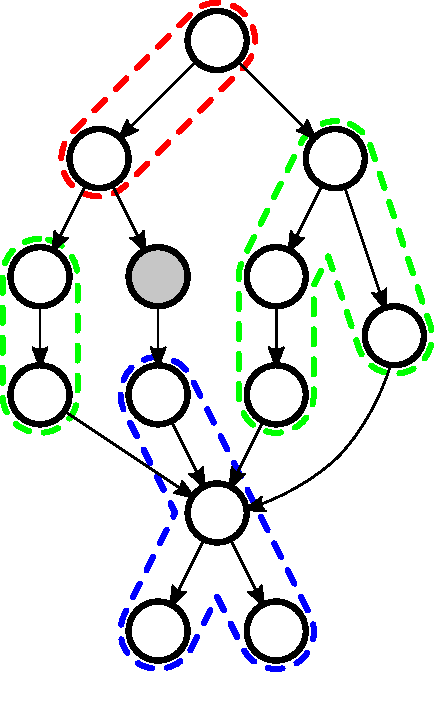
\includegraphics[width=\unitlength,page=1]{figs/graphPartitionsFig.pdf}}%
    \put(0.35075653,1.09704769){\color[rgb]{0,0,0}\makebox(0,0)[lb]{\smash{$\reparamVar_{i}$}}}%
    \put(0.42900388,0.01342784){\color[rgb]{0,0,0}\makebox(0,0)[lb]{\smash{$\mathcal{D}_{i}$}}}%
    \put(0.60518977,1.57213561){\color[rgb]{0,0,0}\makebox(0,0)[lb]{\smash{$\mathcal{U}_{i}$}}}%
    \put(0.73926511,1.38191998){\color[rgb]{0,0,0}\makebox(0,0)[lb]{\smash{$\mathcal{C}_{i}$}}}%
    \put(0.06372864,0.54981535){\color[rgb]{0,0,0}\makebox(0,0)[lb]{\smash{$\mathcal{C}_{i}$}}}%
  \end{picture}%
\endgroup%
\caption{Partitioning a dependency graph into multiple node subsets from the perspective of a random variable node $\reparamVar_i$.}
\label{fig:graphPartitions}
\end{figure}

For any given random choice $\reparamVar_i$, these partitions allows us to factor $W(\reparamVars, \observedVars)$ into three terms:
%%%
\begin{align*}
W_i(\reparamVars, \observedVars)
%
&= \log \frac{p(\xformedVars, \observedVars)}{\guide(\xformedVars | \observedVars)}\\
%
&= \log \frac{p(\mathcal{B}_i)}{\guide(\mathcal{B}_i)} + \log \frac{p( \reparamXform(\reparamVar_i) | \mathcal{B}_i)}{\guide(\reparamXform(\reparamVar_i) | \mathcal{B}_i)}	+ \log \frac{p(\mathcal{D}_i | \reparamVar_i, \mathcal{B}_i)}{\guide(\mathcal{D}_i | \reparamVar_i, \mathcal{B}_i)}\\
%
&= w_i(\mathcal{B}_i) + w_i(\reparamVar_i, \mathcal{B}_i) + w_i(\mathcal{D}_i, \reparamVar_i, \mathcal{B}_i)
\end{align*}
%%%
In the remainder of this section, we prove that the $w_i(\mathcal{B}_i)$ term can be safely removed. Specifically, we prove the following:
%%%
\begin{theorem}
For a discrete random choice $\reparamVar_i$:
\begin{equation*}
\expect_\reparamDist [ \gradparams \log \guide(\reparamXform_i(\reparamVar_i) | \reparamXform(\reparamVars_{<i}), \observedVars) w_i(\mathcal{B}_i) ] = 0
\end{equation*}
\label{thm:wterms}
\end{theorem}
%%%
In proving this theorem, the following two lemmas will be useful:
%%%
\begin{lemma}
\begin{equation*}
\reparamVars_{<i} \cap \mathcal{D}_i = \varnothing
\end{equation*}
\label{lem:depsDisjoint}
\end{lemma}
%
\begin{proof}
By definition, $\reparamVars_{<i}$ are all random choices which occur before $\reparamVar_i$ in program execution order. Also by definition, for all $d \in \mathcal{D}_i$, there exists a path $\reparamVar_i \to d$. As noted above, by construction, this implies that $d$ was created after $\reparamVar_i$ in program execution order. Thus $d$ cannot be in $\reparamVars_{<i}$.
\end{proof}
%%%
%% \paul{in the following proof, the paths mentioned should be from
%%   $\epsilon_i$ rather than $g(\epsilon_i)$? also use $\to$ notation as
%%   above?}
\begin{lemma}
\begin{equation*}
\guide(\reparamXform_i(\reparamVar_i) | \mathcal{B}_i) \equiv \guide(\reparamXform_i(\reparamVar_i) | \mathcal{U}_i \cup \mathcal{C}_i) = \guide(\reparamXform_i(\reparamVar_i) | \mathcal{U}_i)
\end{equation*}
\label{lem:bIndependentFromU}
\end{lemma}
%
\begin{proof}
By construction there is no directed path from $\reparamXform_i(\reparamVar_i)$ to $\mathcal{C}_i$, or vice versa.  Further, all nodes that are upstream of both $\reparamXform_i(\reparamVar_i)$ and $\mathcal{C}_i$ are in $\mathcal{U}_i$ (because all nodes that are upstream of $\reparamXform_i(\reparamVar_i)$ are in $\mathcal{U}_i$ by definition). It follows that these sets are conditionally independent:
\begin{equation*}
\guide(\reparamXform_i(\reparamVar_i), \mathcal{C}_i | \mathcal{U}_i) = \guide(\reparamXform_i(\reparamVar_i)| \mathcal{U}_i) \guide(\mathcal{C}_i | \mathcal{U}_i).
\end{equation*}
Using this, the result is immediate:
\begin{equation*}
\guide(\reparamXform_i(\reparamVar_i) | \mathcal{U}_i \cup \mathcal{C}_i) 
= \frac{\guide(\reparamXform_i(\reparamVar_i), \mathcal{C}_i | \mathcal{U}_i)}{\guide(\mathcal{C}_i | \mathcal{U}_i)} 
= \guide(\reparamXform_i(\reparamVar_i)| \mathcal{U}_i).
\end{equation*}
%\remark{Noah proves this. Is this pretty much just d-separation?}
\end{proof}
%
A corollary of this lemma is that $\guide(\reparamXform_i(\reparamVar_i) | \reparamXform(\reparamVars_{<i}), \observedVars) = \guide(\reparamXform_i(\reparamVar_i) | \mathcal{U}_i)$, since $\reparamVars_{<i}$ must be a subset of $\mathcal{B}_i$.
%%%
We can now prove Theorem~\ref{thm:wterms}:
%%%
\begin{align}
\expect_\reparamDist [ \gradparams \log \guide(\reparamXform_i(\reparamVar_i) | \reparamXform(\reparamVars_{<i}), \observedVars) w_i(\mathcal{B}_i) ]
%
&= \int_\reparamVars \reparamDist(\reparamVars | \observedVars) \gradparams \log \guide(\reparamXform_i(\reparamVar_i) | \reparamXform(\reparamVars_{<i}), \observedVars) w_i(\mathcal{B}_i)\nonumber\\
%
&= \int_{\mathcal{B}_i} \reparamDist(\mathcal{B}_i) w_i(\mathcal{B}_i) \sum_{\reparamVar_i} \reparamDist(\reparamVar_i | \mathcal{B}_i) \int_{\mathcal{D}_i} \reparamDist(\mathcal{D}_i | \reparamVar_i, \mathcal{B}_i) \gradparams \log \guide(\reparamXform_i(\reparamVar_i) | \reparamXform(\reparamVars_{<i}), \observedVars)\nonumber\\
%
\label{eq:wterms_depsDisjoint}
&= \int_{\mathcal{B}_i} \reparamDist(\mathcal{B}_i) w_i(\mathcal{B}_i) \sum_{\reparamVar_i} \reparamDist(\reparamVar_i | \mathcal{B}_i) \gradparams \log \guide(\reparamXform_i(\reparamVar_i) | \reparamXform(\reparamVars_{<i}), \observedVars) \int_{\mathcal{D}_i} \reparamDist(\mathcal{D}_i | \reparamVar_i, \mathcal{B}_i)\\
%
\label{eq:wterms_isDiscrete}
&= \int_{\mathcal{B}_i} \reparamDist(\mathcal{B}_i) w_i(\mathcal{B}_i) \sum_{\reparamVar_i} \guide(\reparamXform_i(\reparamVar_i) | \mathcal{B}_i) \gradparams\log \guide(\reparamXform_i(\reparamVar_i) | \reparamXform(\reparamVars_{<i}), \observedVars) \cdot 1\\
%
\label{eq:wterms_bIndependentFromU}
&= \int_{\mathcal{B}_i} \reparamDist(\mathcal{B}_i) w_i(\mathcal{B}_i) \sum_{\reparamVar_i} \guide(\reparamXform_i(\reparamVar_i) | \mathcal{U}_i) \gradparams \log \guide(\reparamXform_i(\reparamVar_i) | \mathcal{U}_i)\\
%
&= \int_{\mathcal{B}_i} \reparamDist(\mathcal{B}_i) w_i(\mathcal{B}_i) \expect_{\guide} [ \gradparams \log \guide(\reparamXform_i(\reparamVar_i) | \mathcal{U}_i) ]\nonumber\\
%
\label{eq:wterms_zeroexp}
&= \int_{\mathcal{B}_i} \reparamDist(\mathcal{B}_i) w_i(\mathcal{B}_i) \cdot 0 = 0
\end{align}
%%%
Line~\ref{eq:wterms_depsDisjoint} uses Lemma~\ref{lem:depsDisjoint}.
Line~\ref{eq:wterms_isDiscrete} uses the fact that $\reparamVar_i$ is discrete.
Line~\ref{eq:wterms_bIndependentFromU} uses Lemma~\ref{lem:bIndependentFromU} and its corollary.
Finally, line~\ref{eq:wterms_zeroexp} uses Lemma~\ref{lem:zeroexp}. 

We should note that similar methods to our removal of terms from $W$ have been used by prior work to reduce variance in LR gradient estimators. Rao-blackwellization, using the Markov blanket of a node in a graphical model, produces a similar estimator~\cite{BBVI}. In deep generative models, a similar technique allows the derivation of lower-variance estimators for each layer of the deep generative network~\cite{NVIL}. Finally, less conservative (i.e. exact) dependency graphs can be used to reduce gradient variance in stochastic computation graphs~\cite{StochasticComputationGraphs}.

\subsection{Variance Reduction Step 2: Baselines}

Next, we prove that subtracting a constant baseline term $b_i$ from every $w_i$ does not change the expectation in Equation~\ref{eq:finalEstimator}:
%%%
\begin{align*}
\expect_\reparamDist [ \gradparams \log \guide(\reparamXform_i(\reparamVar_i) | \reparamXform(\reparamVars_{<i})) (w_i(\reparamVars, \observedVars) - b_i) ]
%
&= \expect_\reparamDist [ \gradparams \log \guide(\reparamXform_i(\reparamVar_i) | \reparamXform(\reparamVars_{<i})) w_i(\reparamVars, \observedVars) ] - \expect_\reparamDist[ \gradparams \log \guide(\reparamXform_i(\reparamVar_i) | \reparamXform(\reparamVars_{<i})) b_i ]\\
%
&= \expect_\reparamDist [ \gradparams \log \guide(\reparamXform_i(\reparamVar_i) | \reparamXform(\reparamVars_{<i})) w_i(\reparamVars, \observedVars) ] 
\end{align*}
%%%
Where the last step makes use of Lemma~\ref{lem:zeroexp2}.

In our system, we use $b_i = \expect[ w_i ]$, which we estimate with of a moving average of the samples used to compute gradients. While this choice of $b_i$ is not guaranteed to reduce variance, it often does in practice, and previous systems for variational inference and reinforcement learning have exploited it~\cite{BBVI,StochasticComputationGraphs,VarianceReduction}. Another option is to \emph{learn} $b_i$, for example as a neural net function of $\observedVars$~\cite{NVIL}. The proof above also permits $b_i$ to be a function of $\reparamVars_{<i}$ (i.e. all previous random choices), which could reduce variance further by tracking posterior dependencies. This is a promising avenue for future work.

\subsection{Variance Reduction Step 3: Zero Expectation $q$ Factors}

Finally, we prove that we can remove any factors corresponding to discrete (i.e. non-reparameterized choices) from the $\gradparams \log \guide(\xformedVars | \observedVars)$ term in Equation~\ref{eq:hybridEstimator} without changing its expectation:
%%%
\begin{equation*}
\expect_\reparamDist [ \gradparams \log \guide(\reparamXform_i(\reparamVar_i) | \reparamXform_{<i}(\reparamVars_{<i}), \observedVars) ]
%
= \expect_\reparamDist [ \gradparams \log \reparamDist(\reparamVar_i | \reparamVars_{<i}, \observedVars) ]
%
= 0
\end{equation*}
where we have used Lemma~\ref{lem:zeroexp2} and the fact that $\reparamDist = \guide$ and $\reparamXform$ is the identity for discrete random choices.
%%%


\end{document}
